% Vorlage für eine Bachelorarbeit - 2012-2013 Timo Bingmann

% Dies ist nur eine Vorlage. Strikte Vorgaben wie die Bachelorarbeit auszusehen
% hat gibt es nicht. Darum können auch alle Teile angepasst werden.

%\documentclass[12pt,a4paper,twoside]{scrartcl}
%\documentclass[a4paper,12pt,bibtotoc,titlepage, liststotoc,BCOR7mm,headsepline,pointlessnumbers]{scrbook}
\documentclass[a4paper,12pt,titlepage, BCOR7mm,headsepline]{scrbook}
% Diese (und weitere) Eingabedateien sind in UTF-8
\usepackage[utf8]{inputenc}
\usepackage{multirow}
\usepackage{longtable}
\usepackage{tabularx}
\usepackage{numprint}
\usepackage{adjustbox}
\usepackage{graphicx}
\usepackage[T1]{fontenc}
\usepackage{times}
\usepackage{float}
\typearea[current]{current}
%\usepackage{fancyhdr}
\newenvironment{code}{\begingroup\footnotesize \verbatim}{\endverbatim\endgroup}

\addtokomafont{caption}{\small} % Aktive Auszeichnung von Legenden
\setkomafont{captionlabel}{\sffamily\bfseries}
%\bibliographystyle{plain}

% Sprache des Dokuments (für Silbentrennung und mehr)
\usepackage[english,german]{babel}

% Einrückung und Abstand zwischen Paragraphen
\setlength\parskip{\smallskipamount}
\setlength\parindent{0pt}

% Einige Standard-Mathematik Pakete
\usepackage{latexsym,amsmath,amssymb,mathtools,textcomp}

% Unterstützung für Sätze und Definitionen
\usepackage{amsthm}

\newtheorem{Satz}{Satz}[section]
\newtheorem{Definition}[Satz]{Definition}
\newtheorem{Lemma}[Satz]{Lemma}

\numberwithin{equation}{section}

% Unterstützung zum Einbinden von Graphiken
\usepackage{graphicx}

% Pakete die tabular und array verbessern
\usepackage{array,multirow}

% Kleiner enumerate und itemize Umgebungen
\usepackage{enumitem}

\setlist[enumerate]{topsep=0pt}
\setlist[itemize]{topsep=0pt}
\setlist[description]{font=\normalfont,topsep=0pt}

\setlist[enumerate,1]{label=(\roman*)}

% TikZ für Graphiken in LaTeX
\usepackage{tikz}
\usetikzlibrary{calc}

% Hyperref für Hyperlink und Sprungtexte
\usepackage{xcolor}

\usepackage[plainpages=false,pdfpagelabels=false,citecolor=Black, linkcolor=Black]{hyperref} %Verweise werden Links im PDF

% Paket zum Setzen von Algorithmen in Pseudocode mit kleinen Stilanpassungen
\usepackage[ruled,vlined,linesnumbered,norelsize]{algorithm2e}
\DontPrintSemicolon
\def\NlSty#1{\textnormal{\fontsize{8}{10}\selectfont{}#1}}
\SetKwSty{texttt}
\SetCommentSty{emph}
\def\listalgorithmcfname{Algorithmenverzeichnis}
\def\algorithmautorefname{Algorithmus}

%\usepackage{Sweave}
\begin{document}
%\Sconcordance{concordance:bachelorarbeit.tex:bachelorarbeit.Rnw:%
1 74 1 1 0 364 1 1 31 1 2 8 1 1 36 1 2 14 1 1 17 1 2 11 1 1 22 1 2 10 1 %
1 14 1 2 11 1 1 11 245809 0 1 2 6 1 1 13 483890 0 1 2 57 1}


%%%%%%%%%%%%%%%%%%%%%%%%%%%%%%%%%%%%%%%%%%%%%%%%%%%%%%%%%%%%%%%%%%%%%%

\pagestyle{empty} % keine Seitenzahlen
\renewcommand{\thepage}{\roman{page}}

% Titelblatt der Arbeit
\begin{titlepage}

  \begin{center}\large
  \begin{flushleft}
    \quad\includegraphics[height=17mm]{kit_logo_de.pdf} \hfill

    %\includegraphics[height=20mm]{grouplogo-algo-blue.pdf}\quad\null
\end{flushleft}
    \vfill
    \vfill
    \vfill
    \vfill

    Bachelor thesis
    \vspace*{2cm}

    {\bf\huge Evolutionary Hypergraph Partitioning  \par}
    % Siehe auch oben die Felder pdftitle={}
    % mit \par am Ende stimmt der Zeilenabstand

    \vfill

    Robin Andre

    \vspace*{15mm}

    Date: \today 

    \vspace*{40mm}
    \begin{tabular}{rl}
      Supervisors: & Prof. Dr. Peter Sanders \\
      & Dr. Christian Schulz \\
      & M,Sc Sebastian Schlag
    \end{tabular}
    
    \vspace*{10mm}

    %Institut für Theoretische Informatik, Algorithmik \\
    %Fakultät für Informatik \\
    %Karlsruher Institut für Technologie

    \vspace*{10mm}
    % English:
     Institute of Theoretical Informatics, Algorithmics \\
     Department of Informatics \\
     %Karlsruhe Institute of Technology

    \vspace*{12mm}
    \vfill
  \end{center}

\end{titlepage}

%%%%%%%%%%%%%%%%%%%%%%%%%%%%%%%%%%%%%%%%%%%%%%%%%%%%%%%%%%%%%%%%%%%%%%
%%%%%%%%%%%%%%%%%%%%%%%%%%%%%%%%%%%%%%%%%%%%%%%%%%%%%%%%%%%%%%%%%%%%%%

%\vspace*{0pt}\vfill
\ 
\newpage
\clearpage

\section*{Abstract}
The NP-hard hypergraph partitioning problem has many real life applications like processor load balance or VLSI design. As such meta heuristics are the design philosophy to increase solution quality. In this thesis we create an effective evolutionary algorithm 
improving the existing multilevel hypergraph partitioner KaHyPar. We introduce operations heavily integrated in both the evolutionary and multilevel aspect. We evaluate the benefits of the algorithm on 90 instances, showing that the evolutionary component increases solution quality by 2.2\% on average.



\section*{Abstrakt}
Das NP-schwere Hypergraphpartitionierungsproblem besitzt viele Anwendungsgebiete wie Prozessorlastverteilung oder Schaltkreisdesign. Die gängige Strategie ist es Metaheuristiken einzusetzen, um eine Verbessung der Lösungsqualität zu erreichen. In dieser Thesis entwickeln wir einen effektiven evolutionären Algorithmus, der den bestehenden Multilevelpartitionierer KaHyPar verbessert. Wir führen Operationen ein, die sowohl den evolutionären Aspekt als auch den Multilevelaspekt benutzen. Wir evaluieren die Vorteile des evolutionären Algorithmus auf 90 Hypergraphinstanzen, wobei gezeigt werden kann dass eine durchschnittliche Verbesserung von durchschnittlich 2.2\% erzielt werden kann.




\addcontentsline{toc}{chapter}{Abstract}
\selectlanguage{english}
% German and English Abstract
\vfill\vfill\vfill
\ 
\newpage
\clearpage
\ 
\newpage
\clearpage

%%%%%%%%%%%%%%%%%%%%%%%%%%%%%%%%%%%%%%%%%%%%%%%%%%%%%%%%%%%%%%%%%%%%%%
\section*{Acknowledgments}

I'd like to thank Timo Bingmann for the supply of Club-Mate.
\vfill\vfill\vfill
Hiermit versichere ich, dass ich diese Arbeit selbständig verfasst und keine anderen, als die angegebenen Quellen und Hilfsmittel benutzt, die wörtlich oder inhaltlich übernommenen Stellen als solche kenntlich gemacht und die Satzung des Karlsruher Instituts für Technologie zur Sicherung guter wissenschaftlicher Praxis in der jeweils gültigen Fassung beachtet habe.

\bigskip
\vspace*{1cm}
\noindent
Ort, den Datum

\clearpage

%%%%%%%%%%%%%%%%%%%%%%%%%%%%%%%%%%%%%%%%%%%%%%%%%%%%%%%%%%%%%%%%%%%%%%
\tableofcontents
\clearpage
%%%%%%%%%%%%%%%%%%%%%%%%%%%%%%%%%%%%%%%%%%%%%%%%%%%%%%%%%%%%%%%%%%%%%%
\clearpage
%%%%%%%%%%%%%%%%%%%%%%%%%%%%%%%%%%%%%%%%%%%%%%%%%%%%%%%%%%%%%%%%%%%%%%
\mainmatter
\pagestyle{plain}
\chapter{Introduction}
\pagestyle{headings}
\section{Motivation}
A hypergraph is a generalization from a regular graph in the regard that the edges may contain more than 2 vertices.
Many real world scenarios like warehouse article limits, social networks and structures like computer chips can be modeled accurately as a hypergraph but only imprecise as a graph. As a result there are many applications to partition a hypergraph into $k$ blocks in order to analyze or optimize the circumstances translated towards their respective mathematical model. The objective is to minimize the cut between the blocks. Primarily VLSI design is benefitting from hypergraph partitioning in a sense that the amount of interconnected components is bottlenecking the performance and chip size\cite{boese1992high}.  The size of the components also should not be severely disproportionate as this requires longer connections between the components resulting in longer transmission times. \footnote{https://www.nobelprize.org/educational/physics/integrated\_circuit/history/} Therefore the component sizes should be balanced. \newline ~\newline
When trying to maintain balance for the block size hypergraph partitioning is a problem that, similar to balanced graph partitioning, is proven to be NP-hard\cite{garey2002computers}. Since the exact calculation for NP-hard problems is not feasible using the current academic knowledge and state-of-the-art algorithms these problems are often approached using heuristics to improve the corresponding objective while having a practicable runtime. One of the most effective heuristic in regard to graph/hypergraph partitioning is the multilevel paradigm \cite{bulucc2016recent}. By reducing the hypergraph whilst maintaining the hypergraph structure the original problem is translated to an easier problem by a large margin. Therefore a strong initial solution can be created and additionally be improved on during the recreation of the original problem using local search algorithms. While this approach is capable of generating a strong solution within one execution it falls short on further improving this solution due to the limited solution space evaluated. This problem is can be counteracted using meta heuristics such as evolutionary algorithms specifically designed to allow a more efficient traversal of the solution space and avoidance of local optima. 

\section{Contribution}
This thesis augments the existing hypergraph partitioner KaHyPar by adding an evolutionary framework designed to improve on the solution quality generated by KaHyPar. Using ideas presented in the evolutionary graph partitioner KaffPaE, we add new operators to improve the solution quality by evaluating and modifying the structures of solutions generated by KaHyPar in a more effective manner. 
\section{Structure of Thesis}
In the beginning the main focus is to describe precisely how KaHyPar is utilizing the multilevel paradigm to generate the partitions. Afterwards the evolutionary framework is introduced, described and motivated and finally evaluated by comparing the solution quality of the evolutionary algorithm against KaHyPar by partitioning multiple instances using both variants. 
%%%%%%%%%%%%%%%%%%%%%%%%%%%%%%%%%%%%%%%%%%%%%%%%%%%%%%%%%%%%%%%%%%%%%%
\chapter{Preliminaries}
\section{General Definitions}

A hypergraph $H = (V, E, c, w)$ is defined as a set of vertices $V$, a set of hyperedges $E$ where each hyperedge is a subset of the vertices \ e \subseteq V$.

The weight of a vertex is measured by $c: V \rightarrow  \mathbb R_{\ge 0}$. Similarly the weight of a hyperedge is defined by $w: E \rightarrow  \mathbb R_{\ge 0}$. 
The set extension of $c$ and $w$ are defined as $c(V') = \sum_{v \in V'} c(v)$ and $w(E') = \sum_{e \in E'} w(e)$. 
Two verticies $u, v$ are adjacent if $\exists\ e \in E\ |\ u, v \in e$. The vertices in $e$ are called pins. A vertex $u$ is incident to a hyperedge $e$ if $ u \in e$. $I(u)$ is the set of all incident hyperedges of node $u$. The size $|e|$ of a hyperedge $e$ is the number pins in $e$. A $k$-way partition of a hypergraph $H$ is a partition of $V$ into k disjoint blocks $V_1, .., V_k$. $part(u): V \rightarrow [1, k]$ is a function mapping the vertex $u$ into the corresponding partition block.
A $k$-way partition is balanced when $\forall\  1 \le i \le k\ |\ c(V_i) \le (1 + \epsilon) \lceil \frac{c(V)}{k} \rceil $ for a balance constraint $\epsilon$.
A valid solution is a balanced $k$-way partition. An invalid solution is a partition where the balance criterion is not met.
The number of vertices in a hyperedge that are located in $V_i$ are measured by $\Psi(e,V_i) := |\{v \in V_i \ |\ v \in e \}|$. Given a partition $\mathcal{P}$ the connectivity set of a hyperedge e is $\Phi(e, \mathcal{P}) :=  \{V_i\ |\ \Psi(e, V_i) > 0\}$. 
A hyperedge $e$ is a cut edge in a partition $\mathcal{P}$ when $cut(e, \mathcal{P}) := \Phi(e, \mathcal{P}) > 1$. 
Let $\mathcal{E}$ be the set of cut edges from a partition\mathcal{P} The cut metric of\mathcal{P}is defined as $cut(\mathcal{P}) := w(\mathcal{E})$.
The connectivity metric $(\lambda - 1)$ is defined as $(\lambda - 1)(\mathcal{P}) := \sum_{e \in \mathcal{E}}(\Psi(e) - 1)w(e)$.
Both metrics can be used to measure the quality of a solution. We use the connectivity as metric. 

\begin{figure}[t!] 
    \vspace*{-.25cm}
  \centering
   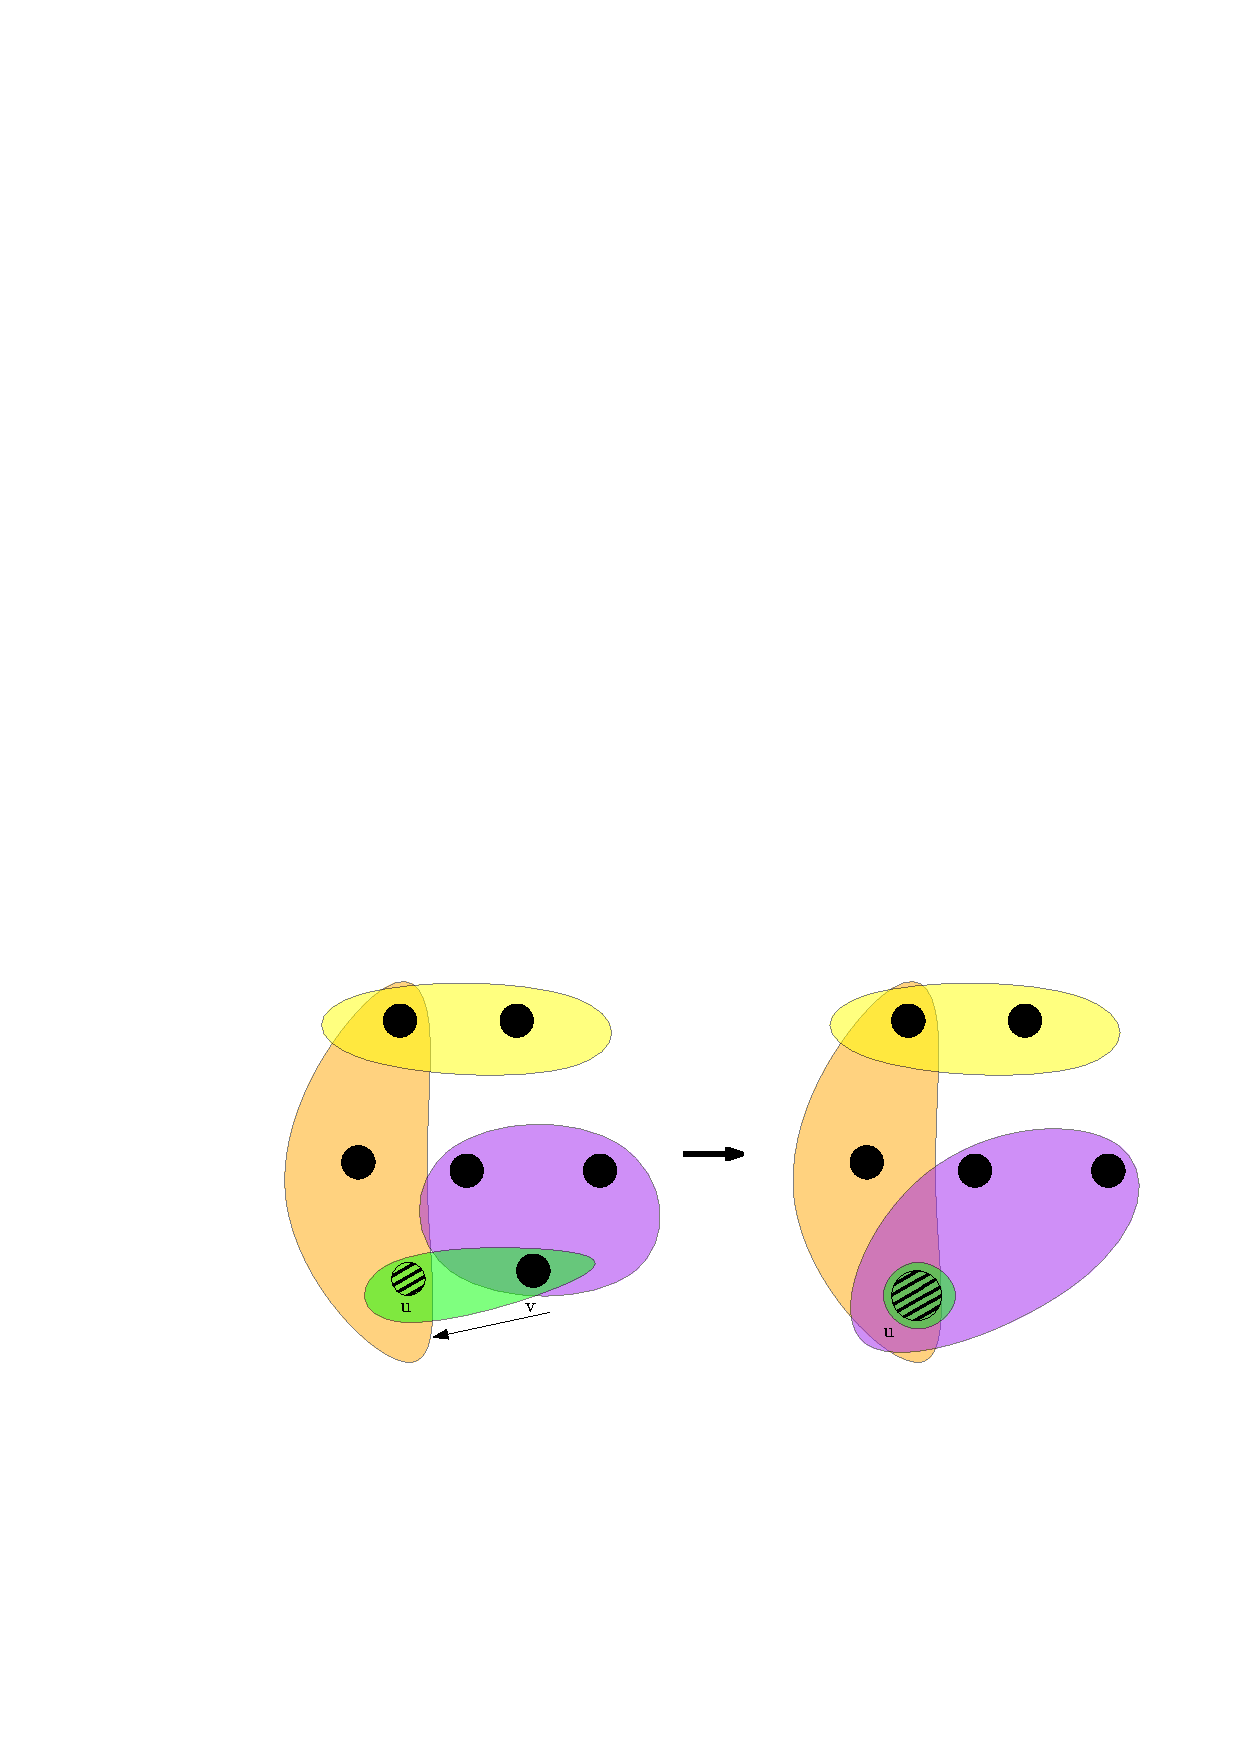
\includegraphics[width=.8\textwidth]{Ipe/Coarsening_Example.pdf}
  \caption{An example of a contraction. Note that the Hyperedges of the reduced node $v$ are rearranged to contain $u$.}\label{fig:coarsening_example}
    \vspace*{-.5cm}
\end{figure}


%Hypergraph := (H;V;E;C)
%Node contraction := 
%Node uncontraction := 
%Net :=
%cut :=
%onnectivity :=
%quality :=
%p%opulation :=
%individual :=
%solution := 
%mbalance:= 

\section{Related Work}
%A Hypergraph cannot be reduced to a graph with clique representation without skewing the cut metric \cite{ihler1993modeling}
%HYPERGRAPH PARTITIONER RELATED WORK BEGIN 
%vvvvvvvvvvvvvvvvvvvvvvvvvvvvvvvvvvvvvvvvv

%NONCITED HYPERGRAPH PARTITIONERS
%UMPa \cite{catalyiirek2013umpa} - multiple constraint
%Hyperswap \cite{yang2016distributed} - partitioning hyperedges instead of vertices
%Cong and Smit \cite{cong1993parallel} - ich weiß nicht mehr warum ich das paper so toll fand
%Panter \cite{trifunovic2008parallel}
% Warum Hypergraphen keine Graphen sind catalyurek1999hypergraph

There are several hypergraph partitioning algorithms, originating from various backgrounds such as processor communication balancing \cite{catalyurek1999hypergraph}, circuit partitioning \cite{alpert1998multilevel} or database storage sharding \cite{kabiljo2017social}.

Two approaches are used for hypergraph partitioning. The first approach is the bisectioning of the hypergraph, where the partition is fixed to $k=2$ as in hMetis\cite{karypis1999multilevel} and MLPart\cite{alpert1998multilevel}. By recursively bisectioning the resulting partitions, $k$ can assume values other than $2$. This is implemented in tools like PatoH \cite{catalyurek1999hypergraph}, Mondrian\cite{vastenhouw2005two} and Zoltan\cite{devine2006parallel}%(allowing imbalanced bipartitions to create partitions of arbitrary k)
. The other approach is to skip the recursion and directly partition the hypergraph into $k$ blocks. This is called a direct $k$-way partition and is used in hMetis-Kway\cite{karypis2000multilevel}, kPatoH \cite{aykanat2008multi} and SHP\cite{kabiljo2017social}(also implementing a recursive bisection). Note that except SHP \cite{kabiljo2017social} all tools are utilizing the multilevel paradigm. 

Of course this is only a collection of the most common hypergraph partitioners, which is why we would like to refer to the surveys \cite{alpert1995recent}\cite{bader2013graph}\cite{papa2007hypergraph}\cite{trifunovic2006parallel}.


% ^^^^^^^^^^^^^^^^^^^^^^^^^^^^^^^^^^^^^^^
% END HYPERGRAPH PARTITIONER RELATED WORK


% EVOLUTIONARY RELATED WORK BEGIN 
% vvvvvvvvvvvvvvvvvvvvvvvvvvvvvvv

Saab and Rao \cite{saab1989evolution} present one of the first evolutionary approaches to hypergraph partitioning by iteratively performing vertex moves comparing the gain to a random threshold using bin pacikgin and iterative improvement. Hulin \cite{hulin1990circuit} presents a genetic algorithm maintaining multiple solutions using a two dimensional representation of circuits and introduce a problem specific crossover operator as well as a mutation operator. A more sophisticated memetic algorithm for the hypergraph partitioning problem was created by Bui and Moon~\cite{bui1994fast}, in which solutions are preprocessed and optimized using the Fiduccia-Mattheyses~\cite{fiduccia1988linear} local search algorithm as well as a new replacement strategy considering the bit-wise difference of the child to the parent partitions for replacement as well as solution quality. 

Chan and Mazmudner\cite{chan1995systolic} provide an genetic algorithm for bipartitioning that assigns better solutions a higher chance to be selected for the crossover operation. The crossover operation splits both input partitions at the same point combining the first split of the first partition and the second split of the second partition.
Areibi \cite{areibi2000integrated} gives another memetic algorithm for the $k$-way hypergraph partitioning problem. Using a variation of FM designed for $k$-way optimization \cite{sanchis1989multiple} local search as well as a 4-point crossover operation, which splits the input partitions at 4 points and alternates between the blocks.
\cite{kim2004hybrid} Kim et al. translate the lock gain local search \cite{kim2004lock} for graphs to hypergraphs and use solution quality and hamming distance as a more potent replacement strategy as well as roulette selection to determine the solutions used in the crossover.
 Sait et al. \cite{sait2006evolutionary} compare the metaheuristics tabu search, simulated annealing and genetic algorithms for $k$-way hypergraph partitioning. Their result is that tabu search is outperforming a genetic algorithm in quality and running time.
Armstrong et al.\cite{armstrong2010investigation} are analyzing the quality and running time performance of parallel memetic algorithms comparing a bounded amount of local search against an unbounded local search stopping only when no improvement can be made. All referenced works that use a crossover operator do so by splitting the input partitions and selecting alternating block fragments.

% ^^^^^^^^^^^^^^^^^^^^^^^^^^^^^ 
% EVOLUTIONARY RELATED WORK END

Sanders and Schulz present an evolutionary framework \cite{sanders2012distributed} for the existing graph partitioner KaFFPa, \cite{holtgrewe2010engineering} introducing different combination and mutation operations for graph partitioning. Their approach uses the mulitlevel paradigm in combination with evolutionary operations.

\section{KaHyPar}


The hypergraph partitioner KaHyPar additionally improves on solution quality optimizing on the connectivity metric using direct $k$-way partitioning \cite{akhremtsev2017engineering} as well as the cut metric using recursive bisection\cite{schlag2016k}.  
KaHyPar also uses a multilevel approach for partitioning see Figure \ref{fig:coarseningexample}. The original hypergraph $H$ is coarsened by repeatedly contracting nodes $u,v$ until either no more contractions are possible or that the minimum amount of nodes required has been reached. The coarsened Hypergraph is referenced as $H_c$. KaHyPar is a n-level algorithm meaning that during each step of the coarsening only one pair of nodes $u, v$ is contracted. All of hyperedges containing $v$ are mapped to $u$ in the process. See Figure \ref{fig:coarsening_example} for an example. 
%TODO explain node selection for coarsening 
On $H_c$ a partitioning algorithm is chosen to generate an initial partitioning for the coarsened hypergraph. Afterwards contraction operations will be reversed and 
during each step of the uncoarsening phase local search algorithms are used to improve the solution quality of $H$. The local search is using a variant of the Fiduccia-Mattheysis algorithm \cite{fiduccia1988linear}. 
\newline
\begin{figure}[H] 
    \vspace*{-.25cm}
  \centering
   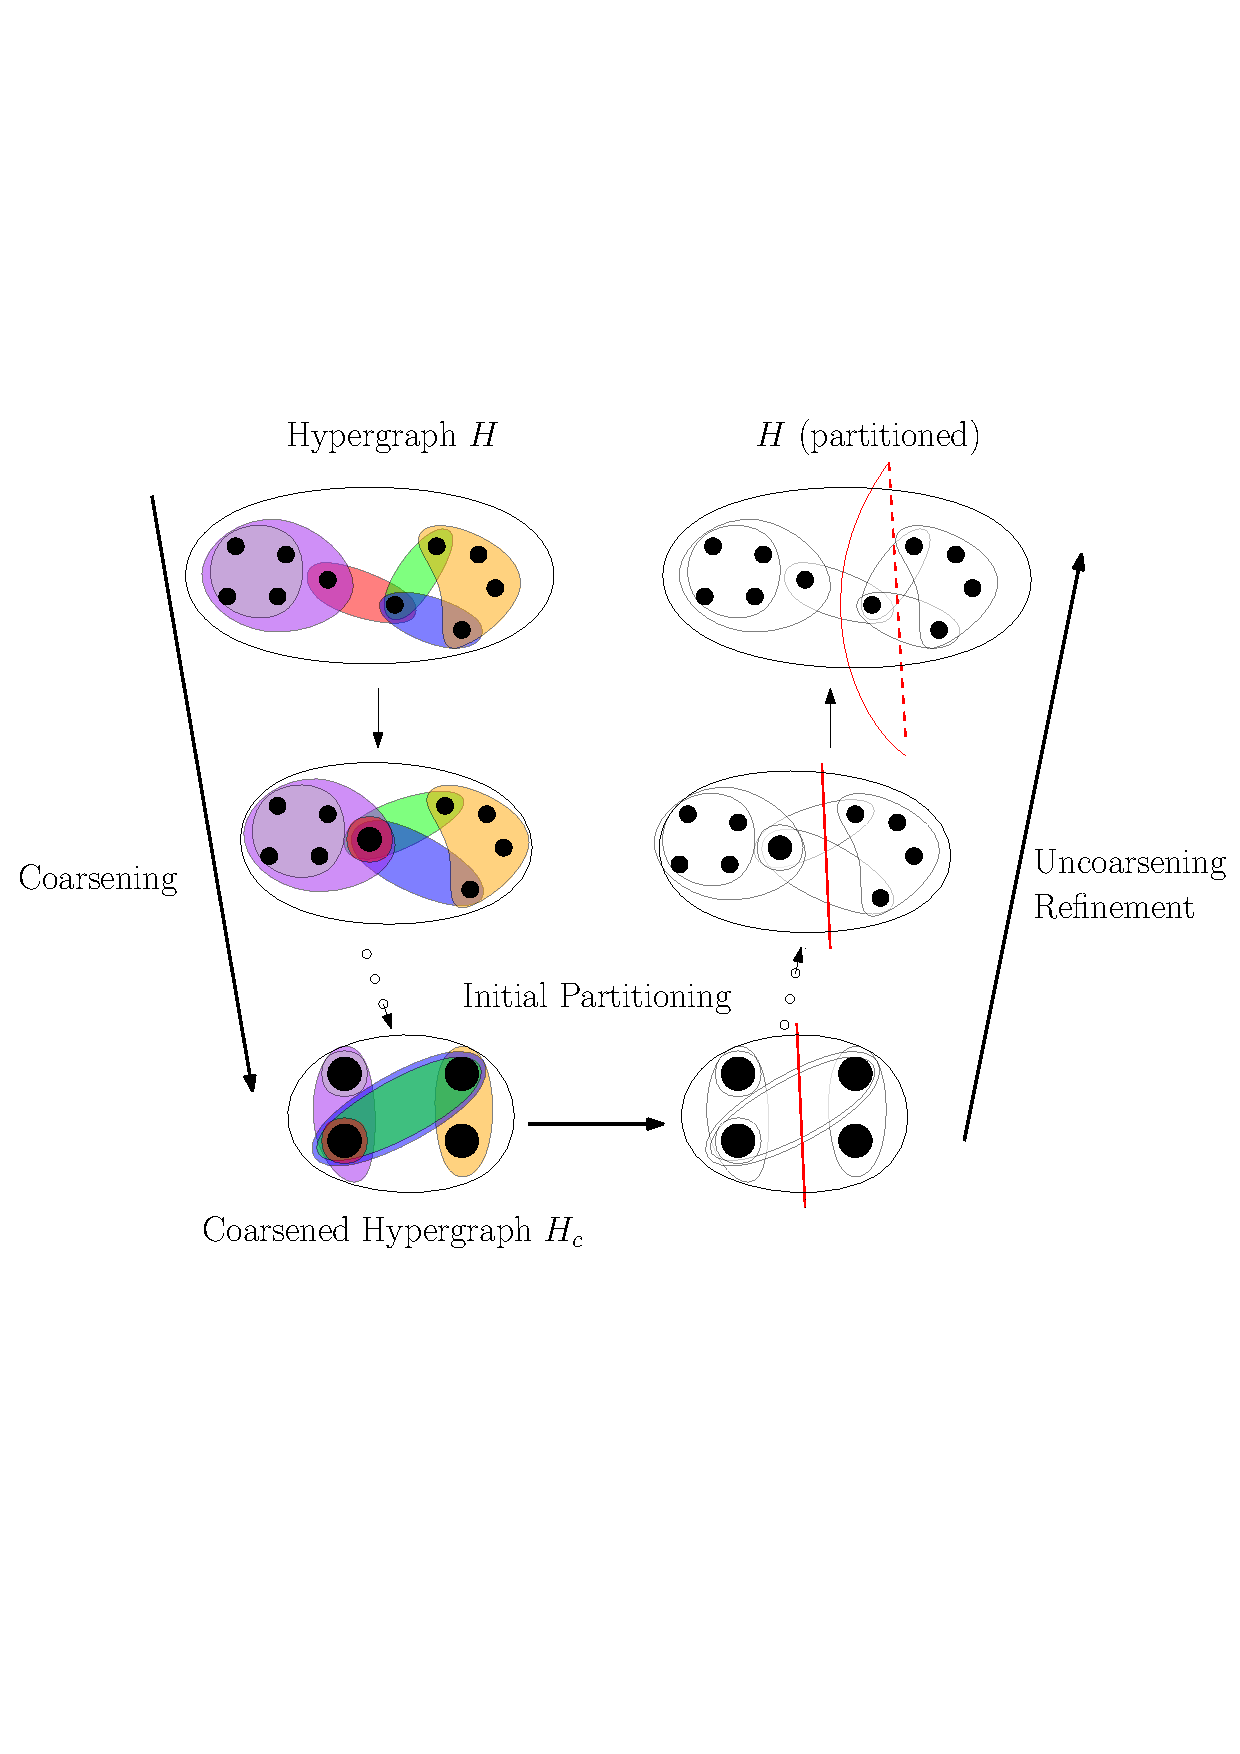
\includegraphics[width=.8\textwidth]{Ipe/Memetic_process.pdf}
  \caption{An example of an iteration. Coarsening, Initial Partitioning and Refinement}\label{fig:coarseningexample} %TODO u nicht gestrichelt; pünktchen
    %\vspace*{-.5cm}

\end{figure}

In 2017 Heuer and Schlag improved KaHyPar by analyzing and exploiting community structures in Hypergraphs \cite{heuer2017improving}, showing that KaHyPar-CA generates solutions of superior quality compared to other established hypergraph partitioners.

%KaHyPar
%KaHiP 
%edge-frequency
%%%%%%%%%%%%%%%%%%%%%%%%%%%%%%%%%%%%%%%%%%%%%%%%%%%%%%%%%%%%%%%%%%%%%%
%TODO only one individual is generated per iteration
%TODO explain evolutionary algorithms, or at least show that this is one
\chapter{KaHyPar-E}
In this chapter we first outline the general procedure of an evolutionary algorithm. Then we transfer the hypergraph partitioning problem onto an evolutionary framework supporting the 
theoretical foundation. Then we introduce operators for combination and mutation as well as strategies for selection and replacement.
\section{Overview}
Evolutionary algorithms are inspired by the theory of evolution. Much like the biological counterpart they attempt to simulate 
an enclosed space where several actors, or individuals, try to compete for survival and reproduction in an isolated setting over the timespan of multiple generations.
The evolution theory states that individuals having more helpful traits like special beaks to assist in aquiring food are more likely to survive longer and 
thus more likely to pass these helpful traits onto the next generation. Addiditionaly some traits occur randomly through changing the genetic information erratically. These are called mutations and are even present in humans, and can be harmful like the sickle-cell desease or beneficial like the ability to consume lactose. In the evolution theory mutations 
are usually a factor that introduces previously nonexistent traits, which would not be able to be recreated using reproduction alone. Repeating the cycle of survival and reproduction the mutations that are helpful will more likely be passed on and established. Based on this principle evolutionary algorithms are essentially converting the process described above onto a mathematical problem. Therefore some initial solutions are generated and then the same steps are repeated until a stopping criterion has been met.
Evolutionary algorithms are usually repeating 4 steps that try to simulate evolution. First some individuals have to be chosen for recombination. Then the chosen individuals have to be combined with each other generating offspring. As third step mutations are performed on some individuals and as fourth step the individuals surviving the iteration(generation) are selected by a corresponding metric, also called fitness. For hypergraph partitioning we consider a partition as an individual and the fitness of said individual is the cut or connectivity metric. We alternate the evolutionary scheme a bit in a sense that we perform combination or mutation exclusively during an iteration and additionally only generate one new solution during said iteration and then replace an existing individual with the new offspring. 

\section{Population}

The algorithm will produce multiple individuals, which are inserted and removed from the population. Only a fixed number of
individuals are in the population. This number is the maximum population size. Further individuals have to compete for a place in the population. 
The population size is an important parameter, as a small value limits the exploration capability and a high value limits convergence \cite{chen2012large}.
We use KaHyPar to fill the initial population. This means that unlike most evolutionary algorithms we use high quality solutions instead of random solutions as initial population.
In order to select a proper population size for the running time we attempt to allocate a fair amount of time towards the creation of the initial population. 
By measuring the duration of one iteration $t_1$ and comparing it to the total running time ${t_{total}}$ we can estimate the amount of iterations $\frac{t_{total}}{t_1}$. Since hypergraph instances
vary greatly in time required to partition, using a fixed population size will most likely be inadequate for most instances. As a solution we try to use a fixed percentage of the total time for generating 
individuals for the initial population. Evaluating the value calculated above we spend approximately 15\% of the alloted time towards creating the initial population and consequently the population size is determined by $0.15*\frac{t_{total}}{t_1}$.
However we introduce lower and upper bounds for the population size to ensure a proper size for evolutionary operators and convergence. That being said the population size has to be at least 3 and 50 at most.
\section{Diversity}
\label{sec:diversity}
%By measuring the difference between two individuals we can gain some knowledge over their internal structure and similarities.
In biological evolution a population with a highly miscellaneous gene pool is considered healty, because the variation between the individuals ensures that no characteristic is carried by every individual and a high perturbation of the gene pool is assured. In that case bad characteristics can be removed through means of reproduction. As reverse conclusion bad characteristics will not be removed if each individual shares said characteristics. 
The same principle is applicable to evolutionary algorithms in a sense that bad characteristics are unable to be removed if they are shared by all solutions. For the hypergraph partitioning problem such a characteristic would be a hyperedge that is also a cut edge in every solution. 

Maintaining diversity is highly recommended\cite{back1996evolutionary}, as it ensures a strong pertubation of the solutions and therefore allows for a greater exploration of the solution scope.
Additionally it prolongs characteristics from manifesting throughout the entire population.
We introduce diversity as a tool for measuring the different characteristics of two individuals. 
As described above the characteristic influencing the quality of a partition are the cut edges. In evolutionary graph partitioning KaffPaE \cite{sanders2012distributed} determines the difference of two partitions P$_1$, P$_2$ by counting the edges that are cut edges in exclusively one of the partitions $cutdiff($P$_1,$P$_2) :=\sum_{e \in E} |cut(e,$P$_1) - cut(e,$P$_2)|$. This approach can be used for hypergraphs, but is not entirely accurate for hypergraphs because cut hyperedges might extend into multiple blocks, see Figure \ref{fig:diversity}. Instead we also count the amount of blocks that are different between the hyperedges $conndiff($P$_1,$P$_2) :=\sum_{e \in E} |\Phi(e,$P$_1) - \Phi(e,$P$_2)|$. This is a more natural representation for the connectivity metric as cut edges.

\begin{figure}[H] 

    \vspace*{-.25cm}
  \begin{center}
   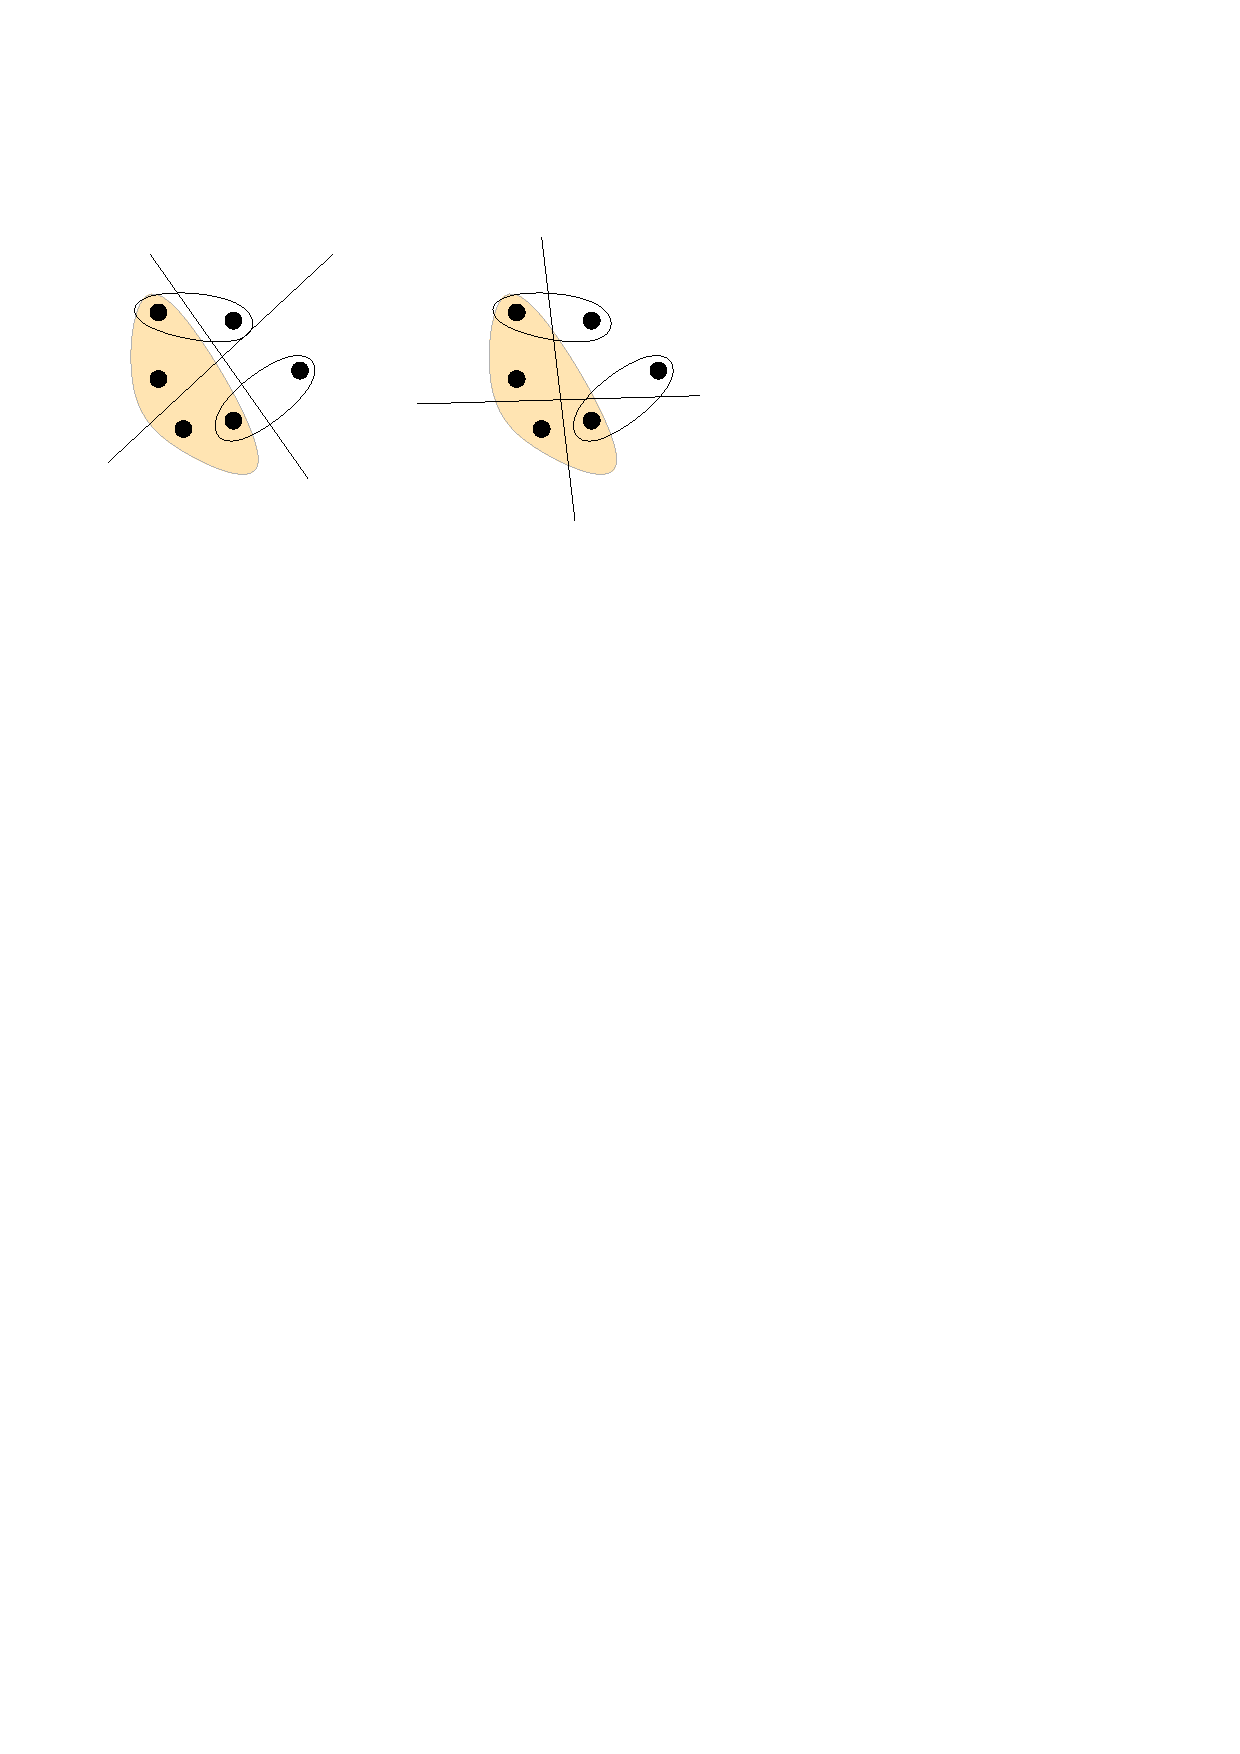
\includegraphics[width=.8\textwidth]{Ipe/connexample.pdf}
  \caption{Two different partitions of the same hypergraph}\label{fig:differentpartitions} 
  \label{fig:diversity}
    %\vspace*{-.5cm}
  \end{center}
  Figure \ref{fig:differentpartitions} shows two different partitions of the same example hypergraph. Since all edges are a cut edge the cut difference is 0. However the partitions are not to be considered equal since the highlighted edge has 
  a different connectivity By using the connectivity difference this issue can be avoided. 
\end{figure}

\section{Selection Strategies}
For an evolutionary algorithm we attempt to generate new, improved solutions by using existing solutions. A logical conclusion is that good individuals have good characteristics that may be passed on to child individuals.
close to the original individual and as result similarly good. We select our individuals using tournament selection \cite{blickle1996comparison}, meaning that the individuals are competing for their chance of recombination by their fitness. In a long term perspective this ensures that good individuals get a more frequent chance of reproduction as stated by the evolutionary theory.  By first selecting two random individuals and using the one with the better solution quality we can extract one individual $I_1$. For operators requiring two seperate Individuals we can simply repeat this step to get a new individual $I_2$. In the unlikely case that the two selected individuals are the same we instead use the worse individual from the second tournament selection.
\section{Combine Operations}
Combine operations generate a new individual by using two or more individuals as input. We present two different combine operators. The first operator C1 combines two partitions which are determined using tournament selection. While C1 uses two parents, the second operator C2 is capable of combining a variable number of X individuals. These individuals are selected from the population by choosing the best X individuals from the population instead of a tournament selection. Both operators use the replacement strategy introduced in section\ref{sec:replacement} to insert the newly generated individuals.
\subsection{Basic Combine (C1)}
\label{sec:basiccombine}
The basic combine uses two parent partitions P$_1$ P$_2$ in order to create a child individual $C$. This is achieved by only allowing contractions of nodes $u, v$ when these nodes are in the same block in both parents. Contractions performed in the same block do not modify the quality of a partition, because the block assignments cannot change, and as a result there is no fluctuation in connectivity for any hyperedge.
This ensures that the solution quality for the coarsened Hypergraph $H_c$ is the same for both parent partitions.  
After the coarsening we do not perform an initial partitioning. Instead we consider the coarsened hypergraph $H_c$ and see which of the parents gives the better objective on $H_c$.
The important part to note is that this operation is different than a V-cycle, since the coarsening condition is more strict due to the consideration of both parents partitions. The uncoarsening and application of local search algorithms which do not worsen solution quality. In combination with using the better partition of the two parents it is ensured that the child solution is at least as good as the best parent solution. \label{qualityassurance} The basic combine is benefitting from highly diverse parent partitions since it passes on more characteristic cut edges, resulting in a more efficient solution exploration. In terms of solution scope the operation is highly convergent due to the quality assurance and strong limitation during the coarsening. 


\subsection{Edge Frequency Multicombine (C2)}
\label{sec:edgefrequency}
We also introduce a multi-combine operator, capable of combining multiple individuals $I_1.. I_n, n \le |P|$ into a new child individual. By analyzing whether an edge $e$ is a cut edge in $I_1 ..I_n$ we can calculate the edge frequency \cite{wichlund1998multilevel} of $e$ by $f(e) := \sum_{i=1}^n cut(e,I_i)$. We use the best $n = \sqrt{|P|}$ individuals from $P$ for determining edge frequency as a standard parameter \cite{delling2011graph}. 
Assuming that the frequent cut edges of the best solutions are most likely a good characteristic, these edges should remain cut edges. By prolonging the contraction of nodes in these frequent cut edges, the other contractions may attach more hyperedges to those nodes. As a result the hyperedges are more probable to become cut edges
 Therefore we penalize contractions of nodes incident to a high frequency edge during the multilevel partition approach by using this formula
\begin{center}
$r(u,v) = \sum_{e \in I(u) \cap I(v)}\dfrac{\mathrm{e}^{-\gamma*f(e)}}{(w(u)w(v))^{1.2}}$ 
\end{center}





to disincentivize early contractions of nodes in edges of high probability. The power of 1.2 on the weight functions is a tuning parameter taken from \cite{delling2011graph} as well as $\gamma = 0.5$.
This rating function is replacing the normal rating function used during the coarsening of KaHyPar. 
The edge frequency operator is not using the input partitions for $H_c$. Instead a new initial partitioning is performed and during the uncoarsening refinement with local search.

%When using this rating function during the coarsening phase of KaHyPar, contractions of high frequency edges are losing up to 40\% in gain calculation using  which is the default parameter from \cite{wichlund1998multilevel}.
Since this operation is generating a new initial partitioning there is no quality assurance opposed to C1.
%\subsection{Basic Combine + Edge Frequency Information}
\section{Mutation operations}
The main objective of mutations is to create more diverse solutions and to improve current solutions to avoid population convergence towards a local optimum.
We propose three different mutation operations. The first operator M1 is intended to increase the solution quality of a partition by reapplying local search algorithms. The second operator M2 is a variation of M1, capable of generating new features. The third operator M3 is intentionally enforcing new characteristics, trying to provide diversity.



%The v-cycle mutations introduced in this chapter are performed on randomly chosen individuals instead of tournament selection. They require one input individual. Stable Net mutation however is using multiple individuals, similar to C1. 
\subsection{V-Cycle (M1)}
A V-cycle is a KaHyPar iteration with the difference that the hypergraph is already partitioned. Similar to the combine operator C1 in section \ref{sec:basiccombine} during the coarsening nodes $u,v$ may only be contracted if $part(u) = part(v)$. Since the hypergraph is already partitioned there is no need for initial partitioning. The main benefit comes from the refinement during the uncoarsening. Due to the randomization factor in the coarsening the structure of the coarsened hypergraph can vary and allow previously unfound improvements during local search.
Using an individual as partition for the hypergraph this operation results in a similar individual $I_{new}$ which has been improved on during the refinement. Due to the fact that neither refinement nor coarsening worsen the quality of the solution $I_{new}$ will have a quality at least equal to $I$. This is a weak mutation and the difference of $I$ and $I_{new}$ is small. This operation will also cause convergence, as multiple applications of a vcycle will eventually no longer improve the solution.
%This operation is also used in KaHyPar-CA + vcycle as the strongest configuration of KaHyPar-CA. However the number of v-cycles performed during one evolutionary iteration is 1, whereas the number of v-cycles performed during one iteration of KaHyPar-CA + vcycle is arbitrarily high to only stop when no further improvements have been found.
\subsection{V-Cycle + New Initial Partitioning (M2)}
Similar to a V-cycle we can coarsen $H$ with a partition limiting the coarsening, but instead of immediately starting the refinement we drop the partition and perform a new initial partitioning on the coarsened hypergraph. This operation pertubes the original more strongly because the vertices are no longer forced to keep their assigned block. Since the partition is
dropped the algorithm used to generate a new partition might produce a worse solution as before. Therefore this operator can create worse solutions and as a result the operator is capable of introducing diversity regardless of current convergence in the population. 
\subsection{Stable Nets (M3)}
Lim et al. \cite{lim1997large} introduce the concept of stable net removal, stating that hyperedges that remain cutedges throughout the iterations are trapping the FM-algorithm in a local minima. Their solution is to force those edges into one block and thus from the cut. 
We use this approach to similarly force recurring cut edges into one block. 
Opposed to the edge frequency operator where the recurring cut edges should remain cut edges, we attempt to force the high frequency edges from the cut.
Again the $\sqrt{|P|}$ best individuals are analyzed, regarding edges most frequent in these solutions. We consider an egde stable if it is in the cut in at least 75\% of individuals inspected.
These edges are then attempted to be forced into the block with the smallest number of nodes in order to maintain the balance criterion. This is done by assigning all nodes $ v \in e$ the block id of the smallest block.
Forcefully moved nodes may not be reassigned to another block by another stable net.
These solutions have most likely siginficantly worse quality. Due to the nature of our selection strategy these solutions are very unlikely to be used in any combine operator. In order to keep these solutions competitive we also perform a vcycle after removing the stable nets. This operator is intended to create individuals with significantly different characteristics. 
\section{Replacement Strategies}
\label{sec:replacement}
Regardless of the operator, the generated individual has to be inserted into the population in order to be used in upcoming iterations. The replacement strategy is the only method of removing an individual from the population.
Therefore the replacement strategy is the driving factor of selection pressure and must maintain a strict environment regarding the fitness of the individuals. 
The naive approach is to remove the worst element from the population and insert the individual in its place, with the intention to ensure a vast majority of the best generated solutions.
The consequence is that the population is rapidly converging towards a local optimum and only covering a small amount of the solution space. Another approach is to replace one of the elements used in the operator. This strategy was originally used for mutations, as the theory behind evolutionary algorithm mutations is to pertubate an existing solution. But this approach neglects fitness and is suboptimal for operators using more than one parent element. 
We use a different strategy maintaining the competitive pressure of the selection whilst also avoiding premature convergence. Similar to the naive approach we consider the fitness of the newly generated individual to replace an individual with worse quality. However we do not replace the worst existing element, instead we replace the most similar element with a worse quality using diversity as measurement for similarity. By only replacing elements of worse quality the population is slowly increasing in quality and converging towards optima. However this approach ensures a more diverse population 
which boosts the combine operator effectiveness and avoids rapid convergence. In fact when considering the population slots rather than the single individual it results in the multiple small convergence lines towards several different local optima while improvements can be made and a convergence towards the best optimum as soon as all slots found a local optimum. 

\begin{figure}[H] 

    \vspace*{-.25cm}
  \begin{center}
   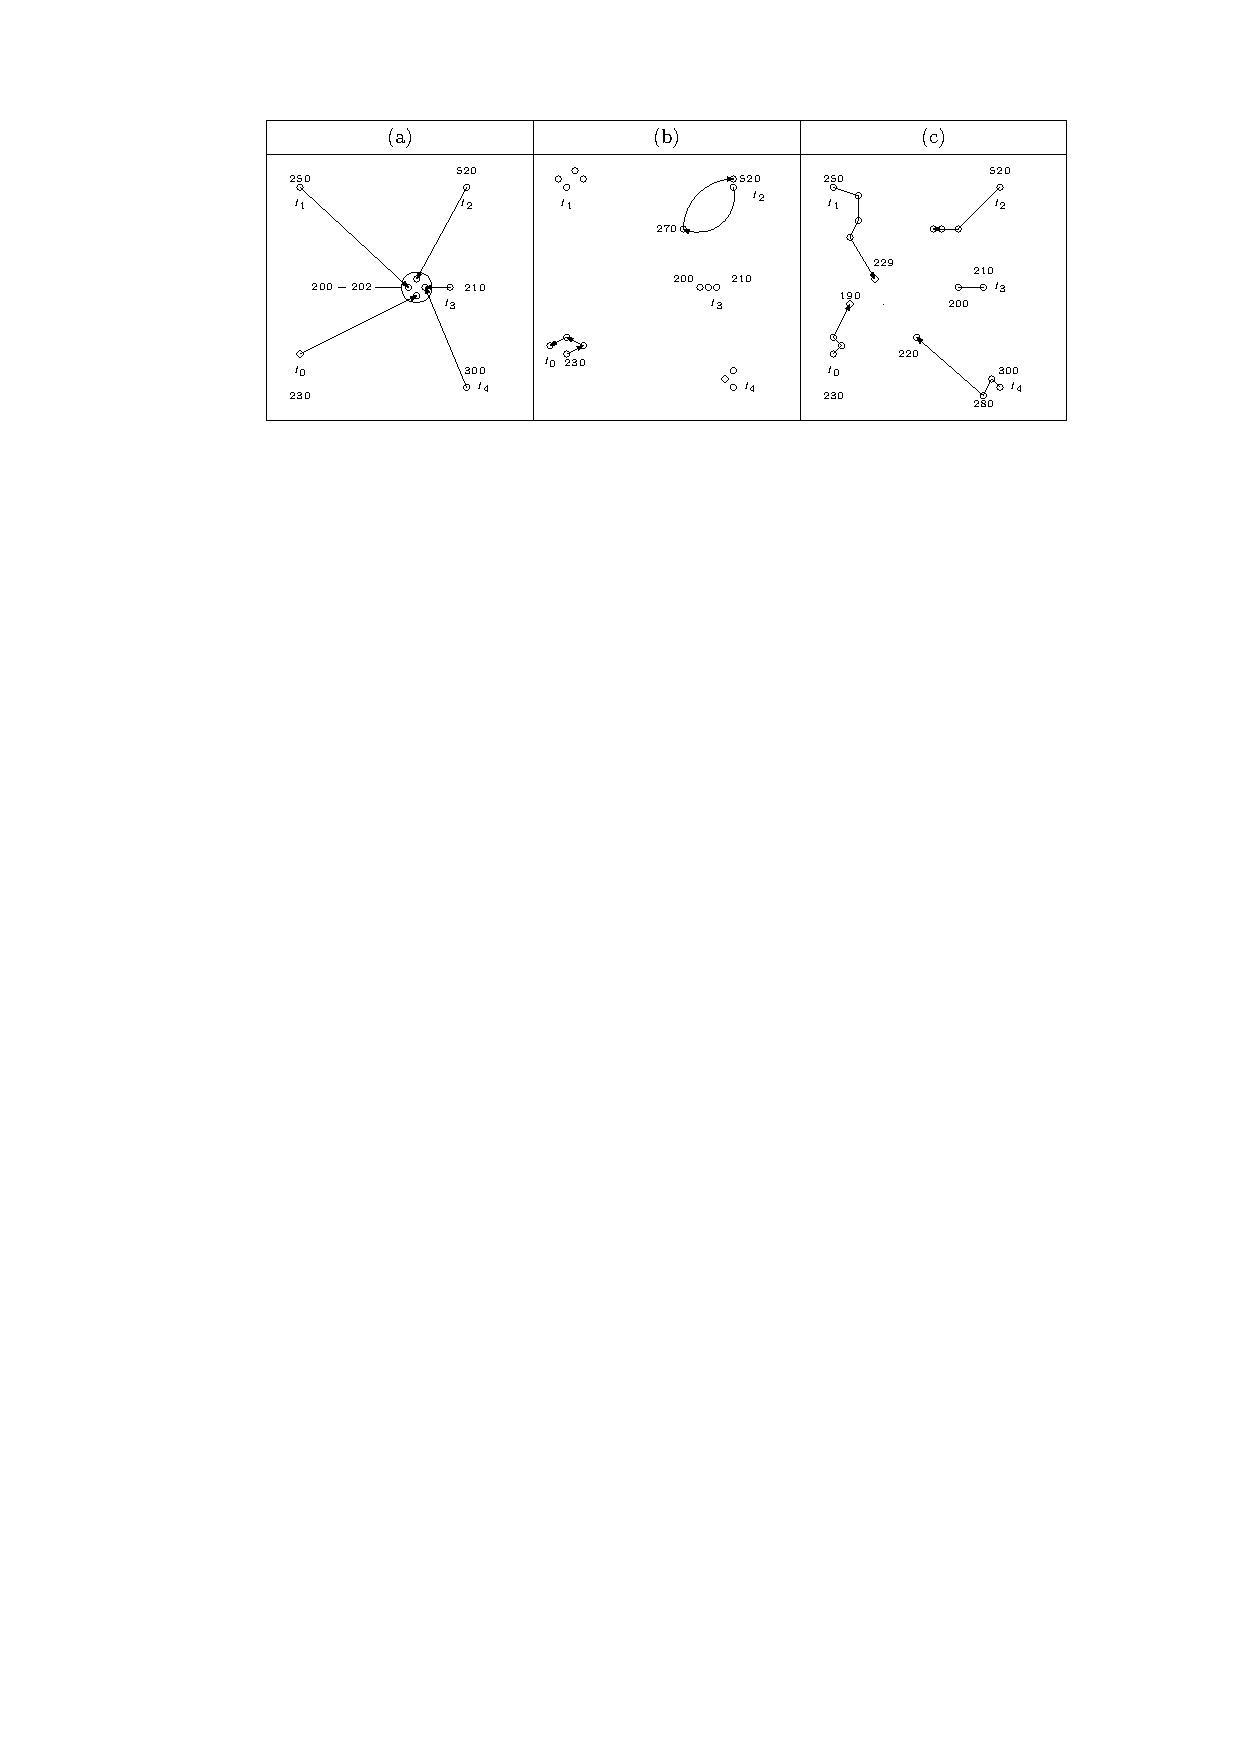
\includegraphics[width=.8\textwidth]{Ipe/diverse_example.pdf}
  \caption{Visual representation of different replacement strategies (a) replacing the worst element, (b) replacing the most similar element \& (c) replacing similar/worse}
  \label{fig:diverse_graphic}
    %\vspace*{-.5cm}
  \end{center}
  In \ref{fig:diverse_graphic} the diversity of the elements is displayed as distance in the 2D plane. The arrows represent whenever an individual is replaced. In (a) a fast convergence towards the local optimum near $I_3$ is happening. Due to the premature convergence and strictness of the replacement strategy there it is highly unlikely that any solution will ever leave this local optimum. In (b) each individual solution is replaced more thoroughly, but good solutions are found at random and may be discarded at any moment. In (c) each of the five slots in the population is slowly converging towards its own respective local optimum, but eventually the best local optimum forces convergence. Note that this graphic is only displaying replacements. The individuals involved in creating these solutions are not linked to the replacement. i.e. $I_3$ at 210 might have been replaced with a solution of quality 200, but the elements creating the solution have been $I_1$ and $I_2$.
\end{figure}

%.....
%%%%%%%%%%%%%%%%%%%%%%%%%%%%%%%%%%%%%%%%%%%%%%%%%%%%%%%%%%%%%%%%%%%%%%
\chapter{Experimental Evaluation}

%#<<test, fig=TRUE, echo=FALSE>>=
%#x = rnorm(100)
%#y = rnorm(100)
%#plot(x,y)
%#@
%Vcycle Mutations
All following plots are using KaHyPar for generating an initial population and perform some of the mentioned operators.
%base with nonevo and random combines




\section{Experimental Setup}
We use two benchmark sets for evaluation. Both sets are using instances from the benchmark set of Heuer and Schlag \cite{heuer2017improving}, which consists of various hypergraphs from the ISPD98 benchmark \cite{alpert1998ispd98}, Sparse Matrices \cite{davis2011university}, the DAC benchmark \cite{viswanathan2012dac} and SAT instances \cite{belov2014proceedings}. 

%The sparse matrices are converted by row-net model \cite{row net model}, whereas the SAT instances are converted to hypergraphs using three approaches \cite{}


%Describe the tuning benchmark set
\newline ~\newline
The first set is called the tuning subset. It consists of 25 Hypergraph instances. The instances were chosen to accurately represent the complete benchmark set. However no instance requiring a high partition time was chosen. This was done to ensure that the instances of the tuning subset can display the effects of the evolutionary algorithm within a smaller time window. The running time for partitions on the tuning subset is 2 hours. The instances were partitioned for $k = 32$ and $\epsilon = 0.03$. Each partitioning run of the tuning subset is repeated 3 times with a different seed for the randomization. This results in 150 CPU-hours required for each data set produced on the tuning subset.
%Describe the benchmark set
\newline

The second set is called the benchmark subset. It consists of 90 Hypergraph instances from the benchmark set. All instances in the benchmark subset were partitioned for $\epsilon = 0.03$ and 7 different values for $k = \{2,4,8,16,32,64,128\}$. The running time for each partitioning on the benchmark subset is 8 hours, and each run is repeated 5 times. This results in 25200 CPU-hours necessary per data set produced on the benchmark subset.
\newline ~ \newline
%Describe why repetitions are performed
The reason for repeating the partitions with different starting seeds is to balance out possible outliers of the randomization. This process is described more detailed in section\ref{the section with the graphic}.
%Describe the reason for using two different sets
The purpose of using two different sets is that the tuning subset is capable of analyzing multiple algorithmic components within a reasonable amount of time, whereas the benchmark subset is able to express more powerful conclusions due to its size.
%Describe the configuration of KaHyPar which we are comparing against
The purpose of this experimental evaluation is to show an improvement of solution quality when comparing the evolutionary algorithm with KaHyPar. (And due to the results of \cite{ein schlag paper} indirectly with other hypergraph partitioning tools)
%Describe KaHyPar-CA-vcycle. 
We compare against KaHyPar-CA, which is an abbrevation for community aware KaHyPar \cite{heuer2017improving}, which uses communities during coarsening to increase the quality of KaHyPar. Additionally KaHyPar-CA can be improved using v-cycles as described in section \ref{sec:vcycles}. Similar to \cite{The work that uses local search unbounded} applying local search until no improvement has been found, KaHyPar-CA can perform v-cycles until no improvement can be found. Such a stopping criterion is implemented in KaHyPar. We set the number of v-cycles to be performed in KaHyPar-CA high enough that the stopping criterion is always met $#v-cycles = 100$. This algorithm configuration is called KaHyPar-CA+V.
%Explain why the number of vcycles is set to 100. Reference the one related work with unbounded improvement
%Describe why KaHyPar has to use repeated repetitions
Neither KaHyPar-CA nor KaHyPar-CA+V are designed to produce multiple solutions within a fixed time. In order to allow a fair comparison with the evolutionary algorithm on the benchmark sets, both KaHyPar-CA and KaHyPar-CA+V are restarted repeadeatly to ensure a proper usage of the running time.
%Reference KaHyPar papers to show that we only have to compare against KaHyPar
\section{Instances \& Methodology}
%Table of instances of the tuning subset
\begin{table}[H]
        \caption{Hypergraph properties of the tuning subset.}
\label{tbl:instancessmall}

\centering
\begin{adjustbox}{max width=\textwidth}
\begin{tabular}{lrrr||l|rrr}
hypergraph & $n$& $m$ & $p$ & hypergraph & $n$ & $m$ & $p$\\
                         \cline{1-4}
                         \cline{5-8}
                         \cline{5-8}
                         \cline{1-4}
                         \cline{1-4}
                         \multicolumn{4}{c||}{ISPD98}          & \multicolumn{4}{c}{SAT14Primal} \\
                         \cline{5-8}
                         \cline{5-8}
                         \cline{1-4}
                         \cline{1-4}

                         ibm06                                 & 32498   & 34826  & 128182 & 6s153                                                & 85646   & 245440 & 572692            \\
                         ibm07                                 & 45926   & 48117  & 175639& aaai10-planning-ipc5              & 53919   & 308235 & 690466   \\
                         ibm08                                 & 51309   & 50513  & 204890& atco\_enc2\_opt1\_05\_21                             & 56533   & 526872 & 2097393  \\
                         ibm09                                 & 53395   & 60902  & 222088& dated-10-11-u                                        & 141860  & 629461 & 1429872  \\
                         ibm10                                 & 69429   & 75196  & 297567& hwmcc10-timeframe & 163622  & 488120 & 1138944  \\
                         \cline{1-4}
                         \cline{1-4}
                         \cline{5-8}
                         \cline{5-8}
                         \multicolumn{4}{c||}{SAT14Dual} & \multicolumn{4}{c}{SPM} \\
                         \cline{5-8}
                         \cline{5-8}
                         \cline{1-4}
                         \cline{1-4}

                         6s133                                 & 140968  & 48215  & 328924  &laminar\_duct3D                                      & 67173   & 67173  & 3833077 \\
                         6s153                                 & 245440  & 85646  & 572692  &mixtank\_new                                         & 29957   & 29957  & 1995041 \\
                         6s9                                   & 100384  & 34317  & 234228  &mult\_dcop\_01                                       & 25187   & 25187  & 193276  \\
                         dated-10-11-u                         & 629461  & 141860 & 1429872 &RFdevice                                             & 74104   & 74104  & 365580  \\
                         dated-10-17-u                         & 1070757 & 229544 & 2471122 &vibrobox                                             & 12328   & 12328  & 342828  \\
                         \cline{1-4}
                         \cline{5-8}
                         \cline{5-8}
                         \cline{1-4}
                         \multicolumn{4}{c||}{SAT14Literal} \\
                         \cline{1-4}
                         \cline{1-4}
                         6s133                                 & 96430   & 140968 & 328924  \\
                         6s153                                 & 171292  & 245440 & 572692  \\
                         aaai10-planning-ipc5                  & 107838  & 308235 & 690466  \\
                         atco\_enc2\_opt1\_05\_21              & 112732  & 526872 & 2097393 \\
                         dated-10-11-u                         & 283720  & 629461 & 1429872 \\
                         \hline\hline
        \end{tabular}
        \end{adjustbox}
        \end{table}
        
Table \ref{tbl:instancessmall} displays the instances in the tuning subset, as well as their basic properties. $n$ is the number of vertices, $m$ ist the number of hyperedges and $p$ is the number of pins. The instances are sorted by their respective classes. 
Similarly table \ref{tbl:instanceslarge} displays the instances of the benchmark subset.
%Table of instances of the benchmark subset
\begin{table}[H]\caption{Hypergraph properties of the benchmark subset.}
\label{tbl:instanceslarge}

\centering
\begin{adjustbox}{max width=\textwidth}
\begin{tabular}{lrrr||l|rrr}
hypergraph & $n$& $m$ & $p$ & hypergraph & $n$ & $m$ & $p$\\
                         \cline{1-4}
                         \cline{5-8}
                         \cline{5-8}
                         \cline{1-4}
                         \cline{1-4}
                         \multicolumn{4}{c||}{DAC2012}    & \multicolumn{4}{c}{SAT14Primal} \\
                         \cline{1-4}
                         \cline{1-4}
                         \cline{5-8}
                         \cline{5-8}
                         superblue19                     & \numprint{522482}                  & \numprint{511685} & \numprint{1713796} & AProVE07-27               & \numprint{7729}   & \numprint{29194}   & \numprint{77124}\\
                         superblue13                     & \numprint{630802}                  & \numprint{619815} & \numprint{2048903} & countbitssrl032           & \numprint{18607}  & \numprint{55724}   & \numprint{130020}\\
                         superblue14                     & \numprint{698339}                  & \numprint{697458} & \numprint{2280417} & 6s184                     & \numprint{33365}  & \numprint{97516}   & \numprint{227536}\\
                         superblue3                      & \numprint{917944}                  & \numprint{898001} & \numprint{3109446} & 6s9                       & \numprint{34317}  & \numprint{100384}  & \numprint{234228}\\
                         \cline{1-4}
                         \cline{1-4}
                         \multicolumn{4}{c||}{ISPD98}    & 6s133                   & \numprint{48215}  & \numprint{140968}  & \numprint{328924}\\
                         \cline{1-4}
                         \cline{1-4}
                         ibm09                           & \numprint{53395}                   & \numprint{60902}  & \numprint{222088}  & 6s153                     & \numprint{85646}  & \numprint{245440}  & \numprint{572692}\\
                         ibm11                           & \numprint{70558}                   & \numprint{81454}  & \numprint{280786}  & atco\_enc1\_opt2\_10\_16  & \numprint{9643}   & \numprint{152744}  & \numprint{641139}\\
                         ibm10                           & \numprint{69429}                   & \numprint{75196}  & \numprint{297567}  & aaai10-planning-ipc5      & \numprint{53919}  & \numprint{308235}  & \numprint{690466}\\
                         ibm12                           & \numprint{71076}                   & \numprint{77240}  & \numprint{317760}  & hwmcc10-timeframe         & \numprint{163622} & \numprint{488120}  & \numprint{1138944}\\
                         ibm13                           & \numprint{84199}                   & \numprint{99666}  & \numprint{357075}  & itox\_vc1130              & \numprint{152256} & \numprint{441729}  & \numprint{1143974}\\
                         ibm14                           & \numprint{147605}                  & \numprint{152772} & \numprint{546816}  & dated-10-11-u             & \numprint{141860} & \numprint{629461}  & \numprint{1429872}\\
                         ibm15                           & \numprint{161570}                  & \numprint{186608} & \numprint{715823}  & atco\_enc1\_opt2\_05\_4   & \numprint{14636}  & \numprint{386163}  & \numprint{1652800}\\
                         ibm16                           & \numprint{183484}                  & \numprint{190048} & \numprint{778823}  & manol-pipe-c8nidw         & \numprint{269048} & \numprint{799867}  & \numprint{1866355}\\
                         ibm18                           & \numprint{210613}                  & \numprint{201920} & \numprint{819697}  & atco\_enc2\_opt1\_05\_21  & \numprint{56533}  & \numprint{526872}  & \numprint{2097393}\\
                         ibm17                           & \numprint{185495}                  & \numprint{189581} & \numprint{860036}  & dated-10-17-u             & \numprint{229544} & \numprint{1070757} & \numprint{2471122}\\
                         \cline{1-4}
                         \cline{1-4}
                         \multicolumn{4}{c||}{SAT14Dual} & ACG-20-5p0              & \numprint{324716} & \numprint{1390931} & \numprint{3269132}\\
                         \cline{1-4}
                         \cline{1-4}
                         AProVE07-27                     & \numprint{29194}                   & \numprint{7729}   & \numprint{77124}   & ACG-20-5p1                & \numprint{331196} & \numprint{1416850} & \numprint{3333531}\\
                         \cline{5-8}
                         \cline{5-8}
                         countbitssrl032                 & \numprint{55724}                   & \numprint{18607}  & \numprint{130020}  & \multicolumn{4}{c}{SPM}\\
                         \cline{5-8}
                         \cline{5-8}
                         6s184                           & \numprint{97516}                   & \numprint{33365}  & \numprint{227536}  & powersim                  & \numprint{15838}  & \numprint{15838}   & \numprint{67562}\\
                         6s9                             & \numprint{100384}                  & \numprint{34317}  & \numprint{234228}  & as-caida                  & \numprint{31379}  & \numprint{26475}   & \numprint{106762}\\
                         6s133                           & \numprint{140968}                  & \numprint{48215}  & \numprint{328924}  & hvdc1                     & \numprint{24842}  & \numprint{24842}   & \numprint{159981}\\
                         6s153                           & \numprint{245440}                  & \numprint{85646}  & \numprint{572692}  & Ill\_Stokes               & \numprint{20896}  & \numprint{20896}   & \numprint{191368}\\
                         atco\_enc1\_opt2\_10\_16        & \numprint{152744}                  & \numprint{9643}   & \numprint{641139}  & mult\_dcop\_01            & \numprint{25187}  & \numprint{25187}   & \numprint{193276}\\
                         aaai10-planning-ipc5            & \numprint{308235}                  & \numprint{53919}  & \numprint{690466}  & lp\_pds\_20               & \numprint{108175} & \numprint{33798}   & \numprint{232647}\\
                         hwmcc10-timeframe               & \numprint{488120}                  & \numprint{163622} & \numprint{1138944} & lhr14                     & \numprint{14270}  & \numprint{14270}   & \numprint{307858}\\
                         itox\_vc1130                    & \numprint{441729}                  & \numprint{152256} & \numprint{1143974} & c-61                      & \numprint{43618}  & \numprint{43618}   & \numprint{310016}\\
                         dated-10-11-u                   & \numprint{629461}                  & \numprint{141860} & \numprint{1429872} & ckt11752\_dc\_1           & \numprint{49702}  & \numprint{49702}   & \numprint{333029}\\
                         manol-pipe-g10bid\_i            & \numprint{792175}                  & \numprint{266405} & \numprint{1848407} & RFdevice                  & \numprint{74104}  & \numprint{74104}   & \numprint{365580}\\
                         manol-pipe-c8nidw               & \numprint{799867}                  & \numprint{269048} & \numprint{1866355} & light\_in\_tissue         & \numprint{29282}  & \numprint{29282}   & \numprint{406084}\\
                         atco\_enc2\_opt1\_05\_21        & \numprint{526872}                  & \numprint{56533}  & \numprint{2097393} & Andrews                   & \numprint{60000}  & \numprint{60000}   & \numprint{760154}\\
                         dated-10-17-u                   & \numprint{1070757}                 & \numprint{229544} & \numprint{2471122} & 2D\_54019\_highK          & \numprint{54019}  & \numprint{54019}   & \numprint{996414}\\
                         ACG-20-5p0                      & \numprint{1390931}                 & \numprint{324716} & \numprint{3269132} & case39                    & \numprint{40216}  & \numprint{40216}   & \numprint{1042160}\\
                         ACG-20-5p1                      & \numprint{1416850}                 & \numprint{331196} & \numprint{3333531} & denormal                  & \numprint{89400}  & \numprint{89400}   & \numprint{1156224}\\
                         \cline{1-4}
                         \cline{1-4}
                         \multicolumn{4}{c||}{SAT14Literal} &                          2cubes\_sphere           & 101492                    & 101492  & 1647264\\
                         \cline{1-4}
                         \cline{1-4}
AProVE07-27              & \numprint{15458}  & \numprint{29194}   & \numprint{77124}    & av41092           & \numprint{41092}  & \numprint{41092}  & \numprint{1683902}\\
countbitssrl032          & \numprint{37213}  & \numprint{55724}   & \numprint{130020}   & Lin               & \numprint{256000} & \numprint{256000} & \numprint{1766400}\\
6s184                    & \numprint{66730}  & \numprint{97516}   & \numprint{227536}   & cfd1              & \numprint{70656}  & \numprint{70656}  & \numprint{1828364}\\
6s9                      & \numprint{68634}  & \numprint{100384}  & \numprint{234228}   & mc2depi           & \numprint{525825} & \numprint{525825} & \numprint{2100225}\\
6s133                    & \numprint{96430}  & \numprint{140968}  & \numprint{328924}   & poisson3Db        & \numprint{85623}  & \numprint{85623}  & \numprint{2374949}\\
6s153                    & \numprint{171292} & \numprint{245440}  & \numprint{572692}   & rgg\_n\_2\_18\_s0 & \numprint{262144} & \numprint{262141} & \numprint{3094566}\\
atco\_enc1\_opt2\_10\_16 & \numprint{18930}  & \numprint{152744}  & \numprint{641139}   & cnr-2000          & \numprint{325557} & \numprint{247501} & \numprint{3216152}\\
        \cline{5-8}
        \cline{5-8}
aaai10-planning-ipc5     & \numprint{107838} & \numprint{308235}  & \numprint{690466} \\
hwmcc10-timeframe        & \numprint{327243} & \numprint{488120}  & \numprint{1138944} \\
itox\_vc1130             & \numprint{294326} & \numprint{441729}  & \numprint{1143974} \\
dated-10-11-u            & \numprint{283720} & \numprint{629461}  & \numprint{1429872} \\
atco\_enc1\_opt2\_05\_4  & \numprint{28738}  & \numprint{386163}  & \numprint{1652800} \\
manol-pipe-g10bid\_i     & \numprint{532810} & \numprint{792175}  & \numprint{1848407} \\
manol-pipe-c8nidw        & \numprint{538096} & \numprint{799867}  & \numprint{1866355} \\
atco\_enc2\_opt1\_05\_21 & \numprint{112732} & \numprint{526872}  & \numprint{2097393} \\
dated-10-17-u            & \numprint{459088} & \numprint{1070757} & \numprint{2471122} \\
ACG-20-5p0               & \numprint{649432} & \numprint{1390931} & \numprint{3269132} \\
ACG-20-5p1               & \numprint{662392} & \numprint{1416850} & \numprint{3333531} \\
\hline
\hline
\end{tabular}
\end{adjustbox}
\end{table}
%Description how the plots are generated
The main interest is to show how the best solution of the population is increasing compared to the time used by the evolutionary algorithm. There are three inherent issues that need to be dealt with. 
\begin{enumerate}
\item The iteration times vary greatly between hypergraphs. 
\item The different seeds need to be normalized.
\item The connectivity also varies greatly between hypergraphs.

\end{enumerate}
To emphasize the first issue, lets assume two hypergraph instances $s$ and $l$. For the small hypergraph $s$ the evolutionary algorithm may perform thousands of iterations, and for the large hypergraph $l$ only 10. When using the absolute time as comparison we have no guarantee how many iterations the evolutionary algorithm has performed in average at a given time point. Similarly when using the iterations of the evolutionary algorithm as comparsion we cannot display the time required by the iterations. The Operator C$_x$ may produce slightly better results than operator C$_y$ per iteration, but also require 1000 times the time per iteration. Sanders and Schulz \cite{sanders2012distributed} present an approach using normalized time as a comparison tool. We choose one of the partitioning algorithms as baseline and determine the average duration $t_I$ to partition a given instance $I$ one time. We then can calculate for each absolute timestamp $t$ of an instance $I$ the normalized time by $t_n = \frac{t}{t_I}$. By doing so we can adjust the variation of iteration times, without dropping the duration information. 

To address the second issue, we used multiple seeds to balance out outlier performance due to randomization. We determine the average best solution for an instance $I$ at the time point $t_n$ as follows. For each seed we create a variable $a_s$ storing the best solution so far. These variables $a_s$ are filled with the first solution created by the corresponding seed. Then the average over all $a_s$ is calculated, determining the first average best solution. Each time a seed $s$ is improving its best solution at a timepoint $t_n$ the corresponding value $a_s$ is updated, and a new average is calculated with the time point $t_n$. This process is illustrated in figure \ref{fig:averagingseeds}. The improvements are processed by ascending order of $t_n$. The result is a list of averaged improvements for Instance $I$, containing elements of the following structure $(avg(a_s), t_n)$. By ordering the list of averaged improvements by $t_n$ we can calculate the average best solution at a timepoint $t_n$.

\begin{figure}[H] 
    
  \begin{center}
   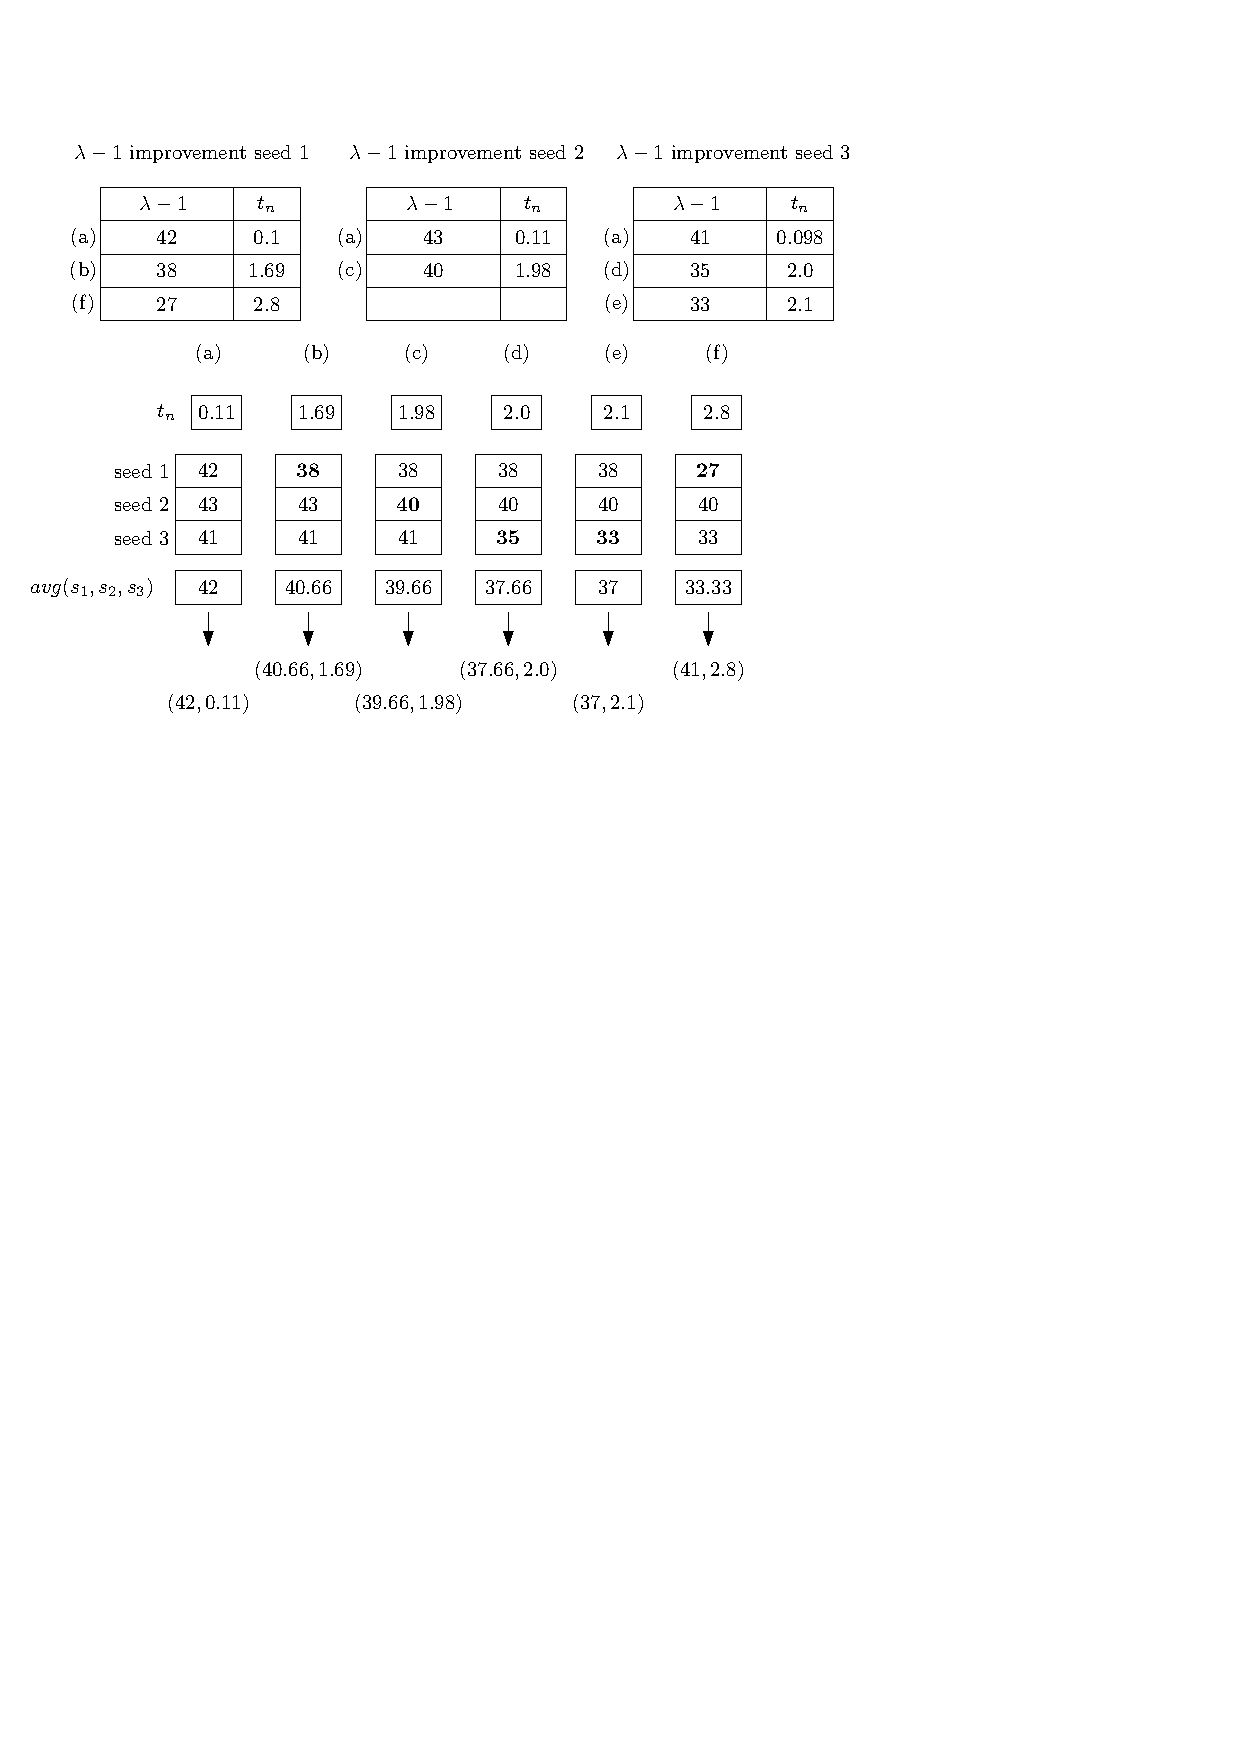
\includegraphics[width=.9\textwidth]{Ipe/seed_averaging_example.pdf}
  \caption{An example for averaging the seeds of an Instance $I$}\label{fig:averagingseeds} %TODO u nicht gestrichelt; pünktchen
  \end{center}
    The solution improvements of the different seeds are run through by ascending normalized time $t_n$ (a)-(f). Then a pair of solution quality and current time is appended to the result every time an improvement is found (b)-(f). The only exception is (a) since there are no existing values to replace. In this case the first values of all seeds are used and the maximum normalized time is used for the first pair.
\end{figure}

Next we need to average the different instances. Because different instances have higly varying connectivity, we cannot use the arithmetic mean as averaging tool. Instead we use the geometric Mean, to counteract a priorization of instances because of their size. Other than that the process is similar to averaging the seeds. For each instance $I$ we create a variable $a_I$ containing the best solution so far. We use the previously generated lists of averaged improvement $l_I$ as input data. Following the same procedure, each time an improvement is found in one of the $l_I$ the corresponding value $a_I$ is updated and a tuple $(geoMean(a_I), t_n)$ is appended to the final result. An example for this procedure can be found in figure \ref{fig:averaginginstances}

\begin{figure}[H] 
    
  \begin{center}
   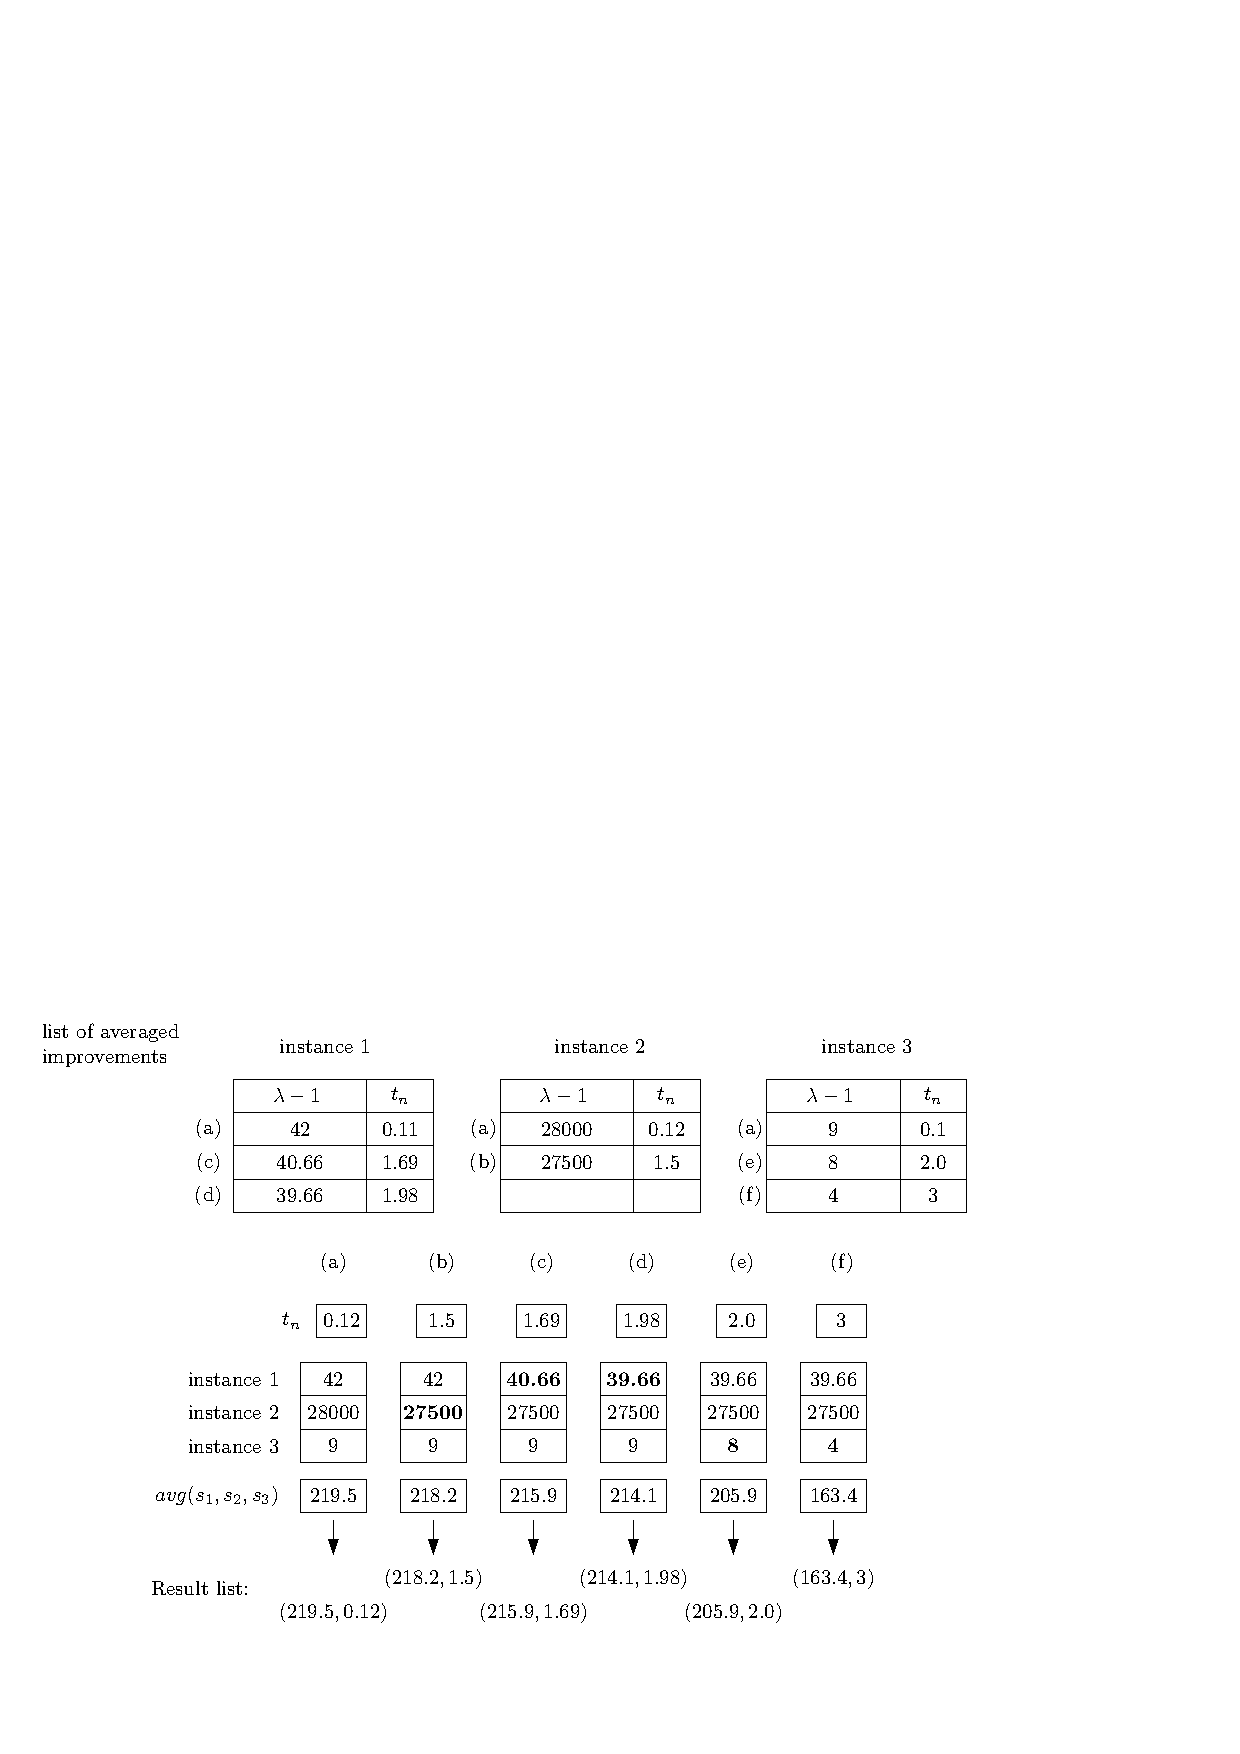
\includegraphics[width=.9\textwidth]{Ipe/instanceaveragingexample.pdf}
  \caption{An example for averaging the seeds of an Instance $I$}\label{fig:averaginginstances} %TODO u nicht gestrichelt; pünktchen
  \end{center}
    Similar to seed averaging the lists of averaged improvement are run through by ascending normalized time $t_n$ (a)-(f). Then a pair of solution quality and current time is appended to the result every time an improvement is found (b)-(f). The only exception is (a) since there are no existing values to replace. In this case the first values of all seeds are used and the maximum normalized time is used for the first pair.
\end{figure}

%Reference to KaffPaE because of normalized time
%Describe why we normalize the time
%Graphic explaining the averaging of the seeds
%Graphic explaining the averaging of the instances
\newpage
\section{First Evaluation} 
All of the data sets presented in this section were created using the tuning subset. These data sets were computed on an Ubuntu 14.04 machine with four Intel Xeon E5-4640 Octa-Core processors @2.4 GHz with 512 GB main memory, 20 MB L3- and 8x256 KB L2-Cache. The following parameters are used as default: Dynamic Population size using $\delta = 0.15$ and $[3,50]$ as lower/upper bound for the population size, $\gamma = 0.5$ as dampening factor for C2, C2 and M3 are using $\sqrt{|P|}$ as default amount of individuals. The threshold of M3 is $0.75$. As preluded the time limit $t$ is set to 2 hours, $\epsilon = 0.03$ and $k=32$. The used seeds are $1,2$ and $3$. The parameters of KaHyPar are set using the default configuration for direct $k$-way partitioning. \footnote{https://github.com/SebastianSchlag/kahypar/blob/master/config/km1\_direct\_kway\_sea17.ini}
% And some on i130 with worse specs
%Say that this is done on the tuning subset
%%REPLACEMENT STRATEGIES
%%vvvvvvvvvvvvvvvvvvvvvv
%First evaluate the replacement strategies
\subsection{Replacement strategy evaluation}
We begin by evaluating the different replacement strategies presented in section \ref{replcaestrategies}. All data sets use KaHyPar-E with the operator C1 as the only evolutionary action. The population size is determined dynamically using $\delta = 15\%$. 
\begin{figure}[H]
\caption{Using different replacement strategies}

\begin{center}
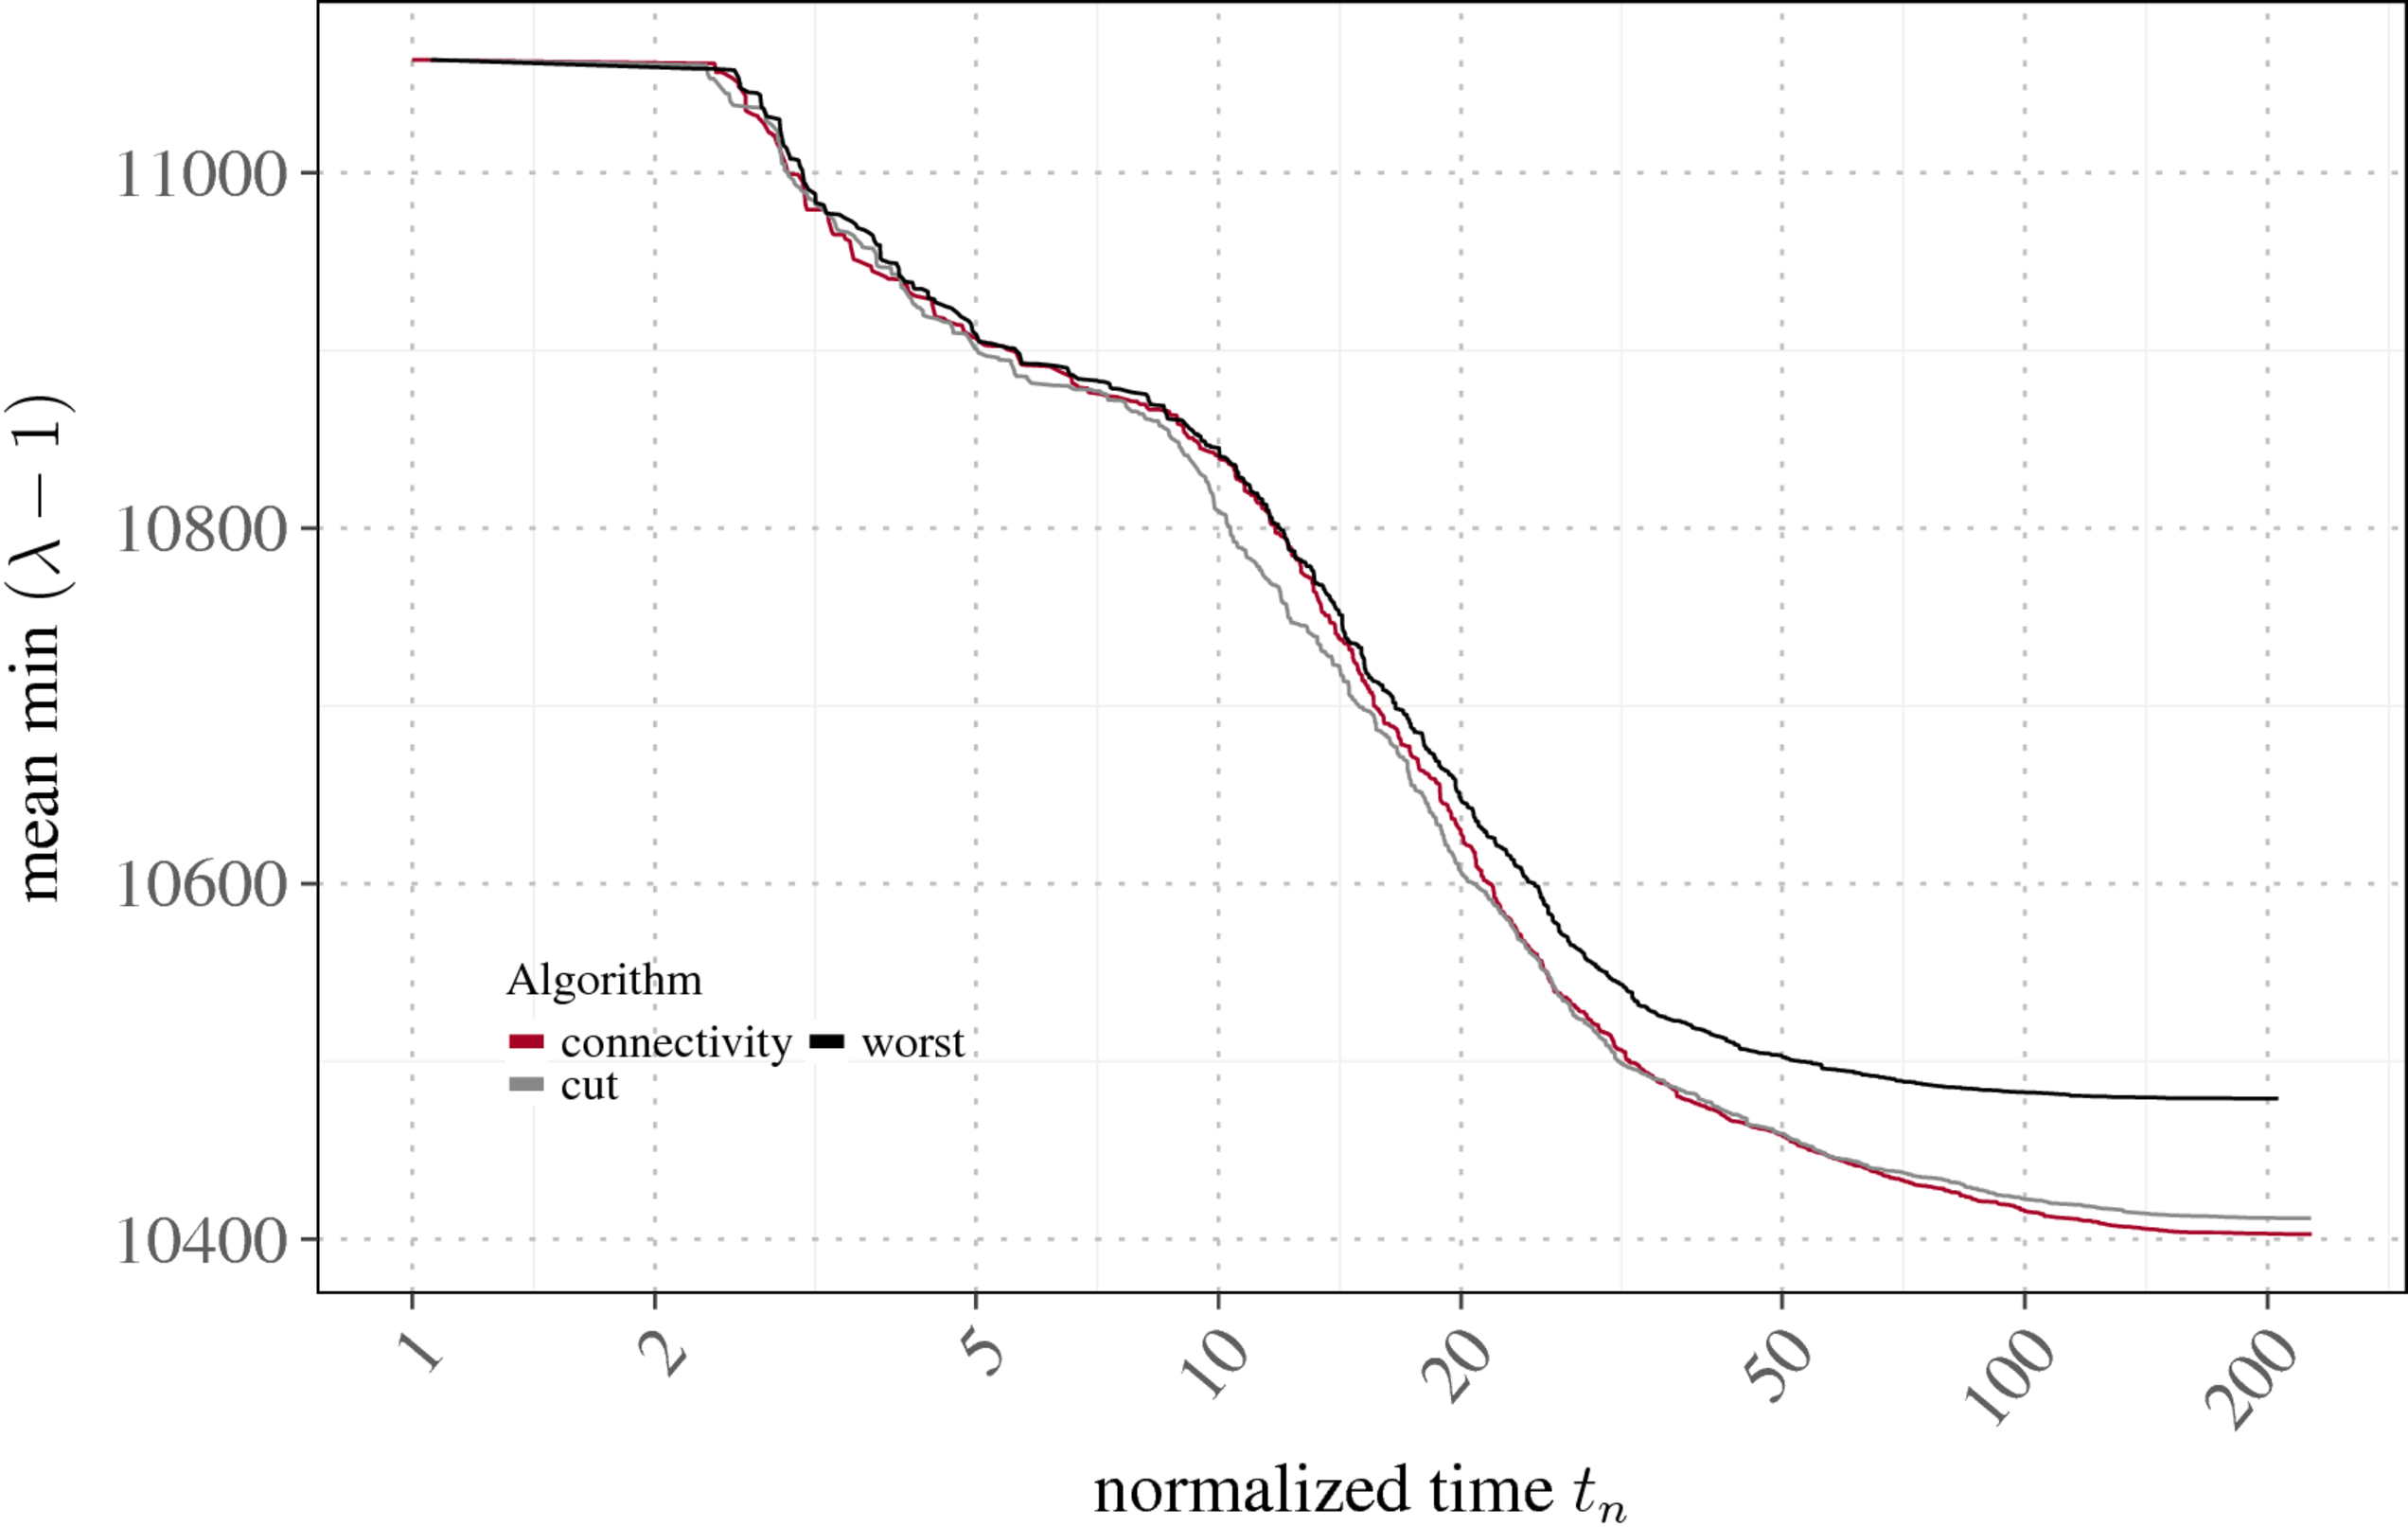
\includegraphics{rnw/tuning_subset_plots/replace_plot-1}\label{fig:replacement}
\end{center}

\end{figure}
In figure\ref{fig:replacement} we compare the effectiveness of the three different replacement strategies. As expected in section \ref{Wo auch immer ich gesagt habe dass worst mist ist} replacing the worst element in the population leads to premature convergence and should be avoided. Using the diversity replacement for graph partitioning \cite{sanders2012distributed} from section \ref{sec:diversity} shows that trying to maintain diversity prevents early plateauing and is thus capable of generating better solutions. However the connectivity approach for diversity is able to slightly increment the solution quality. This comfirms the assumption formulated in section \ref{sec:diversity} that connectivity difference is a more appropriate approach in expressing different characteristics of two partitions. Based on these results we will use connectivity difference as default replacement strategy in all upcoming evaluations.
%Explain why we only use the basic combine operator
%Say that replacing the worst element leads to premature convergence as in section X
%Say that using the connectivity difference is a better approach as cut difference, as expected in section X
%Say that all following plots are using the replacement strategy
%%^^^^^^^^^^^^^^^^^^^^^^
%%REPLACEMENT STRATEGIES
\subsection{Combine operator evaluation}
\label{sec:combineoperatorevaluation}
Next up we evaluate the different combine operators and compare the solution quality against the solution quality of KaHyPar-CA and KaHyPar-CA+V. We evaluate three configurations of the evolutionary algorithm. The specification KaHyPar-E+C$_x$ means that the configuration used the combine operator C$_x$. KaHyPar-E+C1+C2 chooses one of the two combine strategies randomly for each iteration.
%%COMBINE OPERATORS
%%vvvvvvvvvvvvvvvvv
%Explain the algorithms used (KaHyPar C1, KaHyPar C1 C2 KaHyPar C2)
\begin{figure}[H]
\caption{Comparing KaHyPar-E to KaHyPar}
\begin{center}
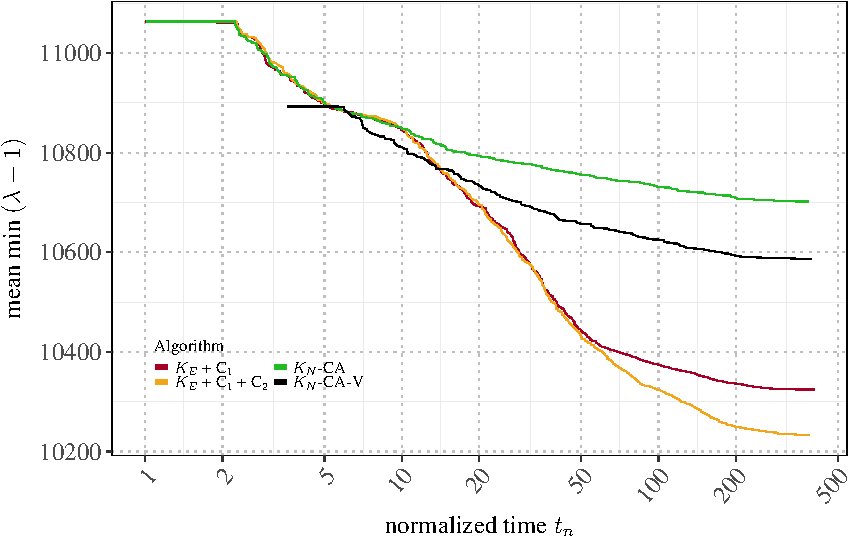
\includegraphics{rnw/tuning_subset_plots/combine_plot-1}\label{fig:combineop}
\end{center} 

\end{figure}
In figure \ref{fig:combineop} we evaluate the results of KaHyPar-E using only basic combines as evolutionary operation against repeated repetitions of KaHyPar-CA and KaHyPar-CA+v which is the strongest configuration for KaHyPar-CA. This evaluation is performed on the tuning subset. The plot lines of KaHyPar-CA, KaHyPar-E + C1 and KaHyPar-E + C1 + C2 are nearly identical up to the time point of 10 $t_n$ normalized time. This is due to the fact that KaHyPar-E is using KaHyPar-CA to generate the initial population. The variations are caused by hardware limitations causing minor fluctuation in the time for performing an iteration and thus slight variations in the normalized time. However the values generated are the same since KaHyPar-CA is configured with the same seed during each of those experiments. KaHyPar-CA+v is not sharing the same starting curve. Since v-cycles are time consuming the algorithm steps of KaHyPar-CA+v are slower than the steps of KaHyPar-CA, resulting in an offset of the starting point for the plot line. As expected KaHyPar-CA+v produces better solutions than KaHyPar-CA, which also extends to repeated repetitions. Both variations of KaHyPar-E gain a significant amount of improvement after generating the initial population. This is due to the combine schemes being able to exploit structural improvements by comparing different partitions as described in \ref{sec:basiccombine} and continually improving the solution quality by the assurance of nondecreasing solution quality \ref{qualityassurance}. However this operation is eventually converging into a local optima since all individuals are going to be replaced with the best solution in relatively close proximity due to the replacement strategy, and neither replacement strategy nor operator are capable to decrease the solution quality of a given individual. the multicombine operation C2 however is not restricted to this assurance. This operator is profiting from a stable population in a sense that the best solutions in the population can most likely be considered good solutions. This is visible in the plot since KaHyPar-E + C1 + C2 is not drastically different from KaHyPar-E + C1 while the basic combine is still effective but allows for an improvement of solution quality whereas KaHyPar-E + C1 is plateauing. Comparing KaHyPar-E + C1 against KaHyPar-CA + v using the Wilcoxon-Pratt Test generates a $Z$-Value of 4.37 indicating that KaHyPar-E + C1 is computing better solutions with a confidence of 99.9998\%.
%%^^^^^^^^^^^^^^^^^
%%COMBINE OPERATORS
%%MUTATION OPERATORS
%%vvvvvvvvvvvvvvvvvv
\subsection{Mutation operator evaluation}

\begin{figure}[H]
\caption{Different Mutation Operations}
\begin{center}
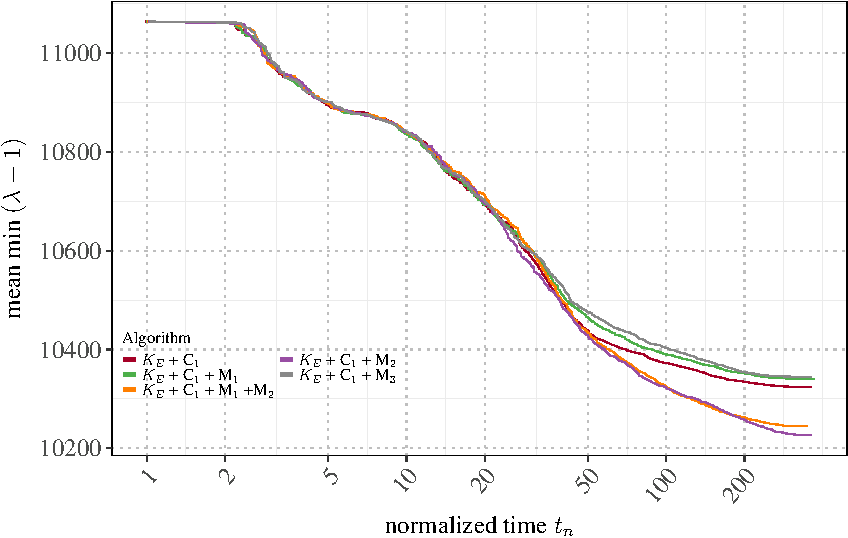
\includegraphics{rnw/tuning_subset_plots/mutation_plot-1}
\end{center}

\end{figure}
In this figure the effectiveness of the different mutation operators are evaluated. Each data set was created using a 50\% chance of C1 and a 50\% chance of the respective mutation operations. In the specific case M1 + M2 the mutation operation performed was selected uniformly at random. This evaluation was performed on the tuning subset. Adding simple v-cycles M1 to the already existing combine operator is in fact performing worse. This is due to the fact that v-cycles share the same quality assurance as C1 and are thus unable to create worse solutions which are necessary to broaden the solution scope of the population. Individuals that have been optimized during the execution of the algorithm also often have been improved by v-cycles or already have a good enough quality so that v-cycles cannot find improvements. In conclusion this means that v-cycles alone are unable to prevent premature convergence. In contrast using v-cycles with new initial partitioning M2 or a combination of both mutation operators will generate better solutions. Since M2 is not limited by the quality assurance of C1 and M1, worse solutions can be created and the solution scope can be explored more effectively. Stable net detection M3 is generating worse solutions or using up more time to generate individuals and therefore dropped from the algorithm. Interestingly when considering how often the different mutation operations have been able to generate a new best solution M3 has only been able to do so for 2 instances out of 25 whereas any combination of M1 and M2 have created a new best solution in all 25 instances. This suggests that M3 is an operation depending on the hypergraph structure and not easily applicable to a generic hypergraph. Due to the replacement strategy newly generated solutions are only considered for insertion if the solution quality is better than the worst individual in the population and will lead to convergence regardless of which mutation operators are applied. 



%%^^^^^^^^^^^^^^^^^^
%%MUTATION OPERATORS

%%DIFFERENT REPLACEMENT OPERATORS FOR MUTATIONS
%%vvvvvvvvvvvvvvvvvvvvvvvvvvvvvvvvvvvvvvvvvvvvv
\subsection{Mutation replacement strategies}


Mutation operations can be inserted into the population in two different ways. Replacing the element used for the mutation in the classical sense of evolutionary algorithms, or using the diversity replacement approach. We evaluate whether the different replacement strategies are influencing the solution quality.
\begin{figure}[H]
\caption{Different replacement strategies for mutations}
\begin{center}
%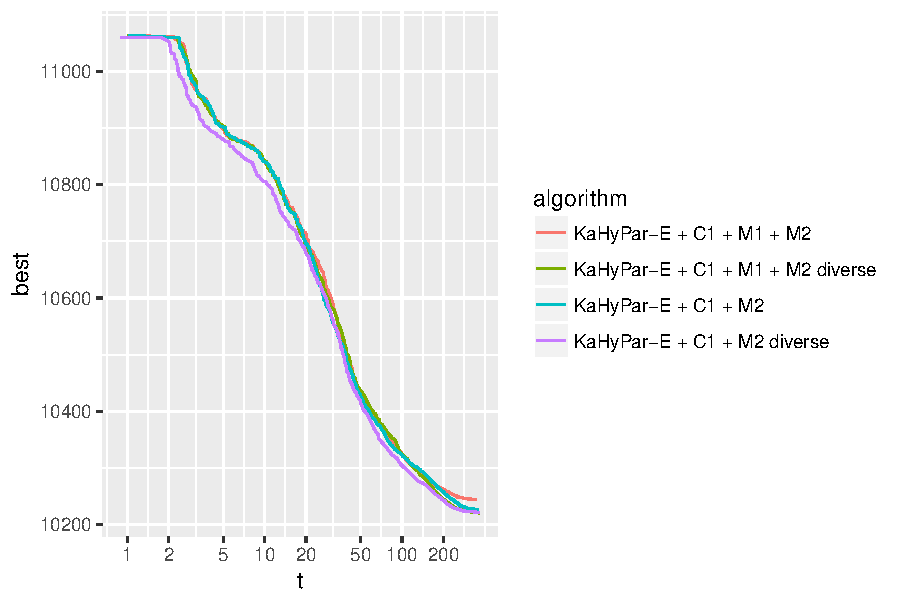
\includegraphics{bachelorarbeit-insertrandom}
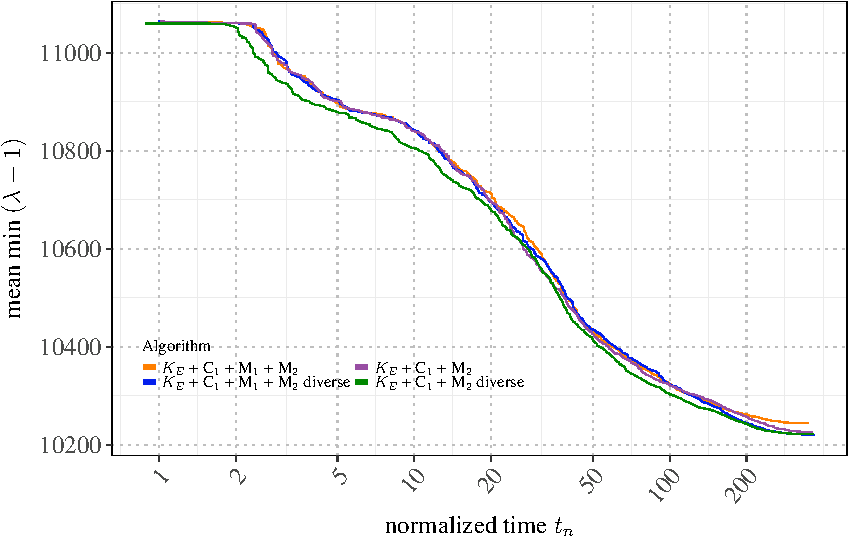
\includegraphics{rnw/tuning_subset_plots/diverse_plot-1}

\end{center}
As seen in this plot the different replacement strategies are displayed for M2 and a combination of M1 and M2. While the difference in KaHyPar-E + C1 + M2 and KaHyPar-E + C1 + M2 diverse is only a miniscule improvement in convergence time and solution quality, the difference of KaHyPar-E + C1 + M1 + M2 and KaHyPar-E + C1 + M1 + M2 + diverse is more prominent in terms of solution quality.

\end{figure}
%Say that using diverse replacement is good
%%^^^^^^^^^^^^^^^^^^^^^^^^^^^^^^^^^^^^^^^^^^^^^
%%DIFFERENT REPLACEMENT OPERATORS FOR MUTATIONS
\section{Tuning Parameters}
KaHyPar-E is adding the following parameters to KaHyPar: dynamic population size $\delta = 0.15$, upper and lower bound limits for the population size $[3,50]$, the edge frequency dampening parameter $\gamma = 0.5$ as well as the amount of individuals used by C2 \& M3 $n = \sqrt{|P|}$. Additional parameters are the replacement strategy, as well as the distribution of combine operators and mutation operators. Most importantly, KaHyPar-E adds the time limit $t$. Noteworthy parameters of KaHyPar include $\epsilon = 0.03$, $k$ and the seed $s$. For other parameters of KaHyPar we refer to the default configurations \footnote{https://github.com/SebastianSchlag/kahypar/blob/master/config}. 
\subsection{Combine chance distribution}
As seen in section \ref{sec:combineoperatorevaluation} a combination of both C1 + C2 is generating better results when being used together. We want to analze different percentages regarding the distribution of the two operatos
\begin{figure}[H]
\caption{Edge frequency chance}
\begin{center}
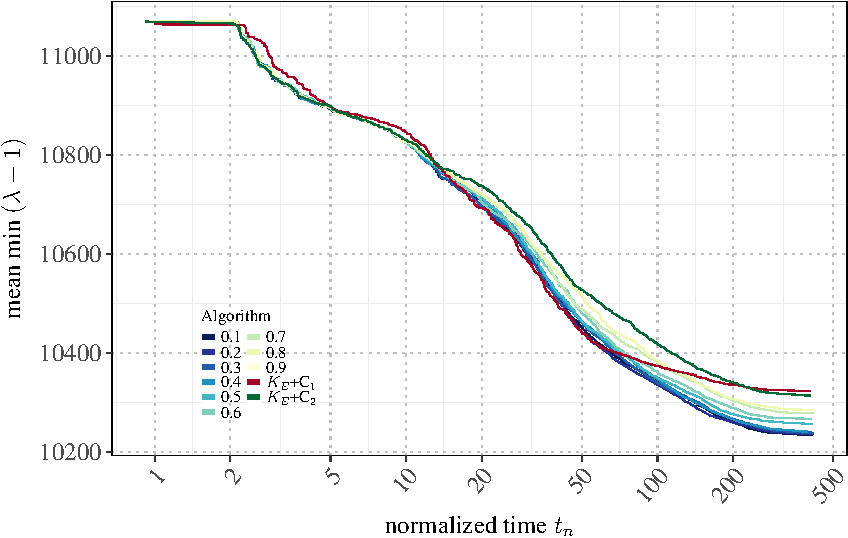
\includegraphics{rnw/tuning_subset_plots/edge_tuning_plot-1}
\end{center}
In this plot the chances of performing an edge frequency instead of a basic combine are displayed. Clearly recognizable is that a proper application of both operators will lead to improvements. The optimal values are in a range from 20\% to 50\%, however similar to the mutation chance tuning no significant difference can be observed between the tuned values.  
\end{figure}
Additional parameters for that were used as default configuration. The dampening factor for edge frequency (C1) is set to $\gamma = 0.5$ as in \cite{wichlund1998multilevel}. The time allocation for creating the population is set to 15\% of the total time. The time limit was set to 8 hours on the benchmark subset and 2 hours on the tuning subset.



\subsection{Mutation chance distribution}
The parameter spectrum of the evolutionary algorithm is rather voluminous. Beginning with the different chances of the combine and mutation operations to be chosen. As such we first evaluate the operations themselves before tuning the respective chances. The first chance is the amount of mutations performed in contrast to combinations. As such the best value for mutation chance using new initial partitioning, the most powerful mutation operation results in a value of 40\% to 50\% for mutation chance. This is drastically diverging from the chance used in evolutionary graph partitioning which is around 10\% \cite{sanders2012distributed}. 
\begin{figure}[H]
\caption{New initial partitioning mutation chance}
\begin{center}
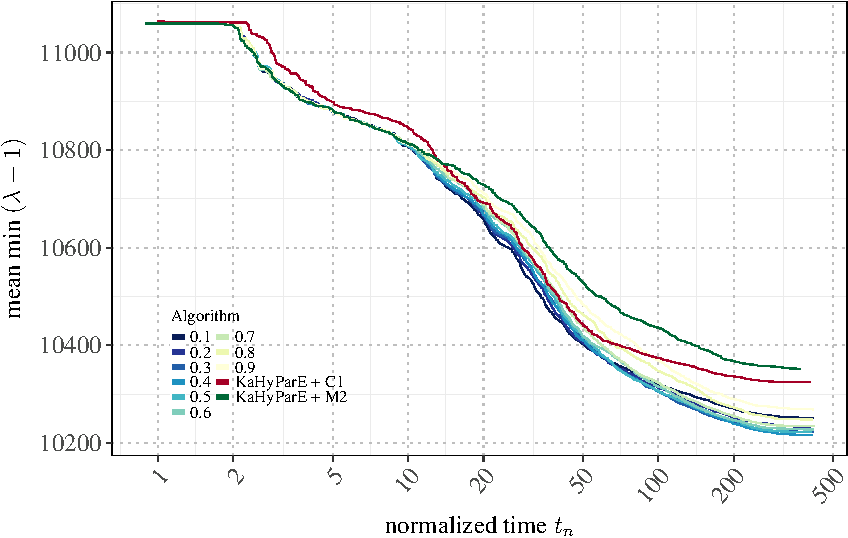
\includegraphics{rnw/tuning_subset_plots/mutation_tuning_plot-1}
\end{center}
In this plot the different mutation chances are represented. The percentages represent the chance of performing a new initial partitioning vcycle. If not performing a new initial partitioning a basic combine is performed. It is visible that choosing either 0\% mutation chance or 100\% mutation chance are both not viable for generating good solutions. A combination of both operators is increasing solution quality. As seen in this experiment a mutation chance of 30\% -50\% for new initial partitioning is generating the best solutions. This experiment was performed on the tuning subset to generate values for the run on the benchmark subset.
\end{figure}
\section{Final Evaluation}
Now we use the results form the tuning subset and translate them onto the benchmark subset. As already mentioned the data sets are generated over more hypergraph instances, using $t$ 8 hours for partitioning, $\epsilon = 0.03$, and $\k = \{2,4,8,16,32,64,128\}$. The following data sets are evaluated on the benchmark subset: KaHyPar-CA, KaHyPar-CA-V, KaHyPar-E+C1, KaHyPar-E+C1+C2 and KaHyPar-E+M1+M2. The data sets were created on a cluster consisting of 512 16-way Intel Xeon compute nodes. All nodes contain two Octa-core Intel Xeon processors E5-2670 (Sandy Bridge) @ 2.6 GHz and have 8x256 KB of level 2 cache and 20 MB level 3 cache. Each node has 64 GB of main memory and local disks with 2 TB capacity. The nodes were allocated exclusively to avoid cpu time interference.
%List Configuartions for final evaluation
%Convergence plot for all k
%Convergence plot split by k 
%Improvement Table
%Performance Plot
% => Convergence all
\begin{figure}[H]
\caption{Benchmark subset results}
\begin{center}
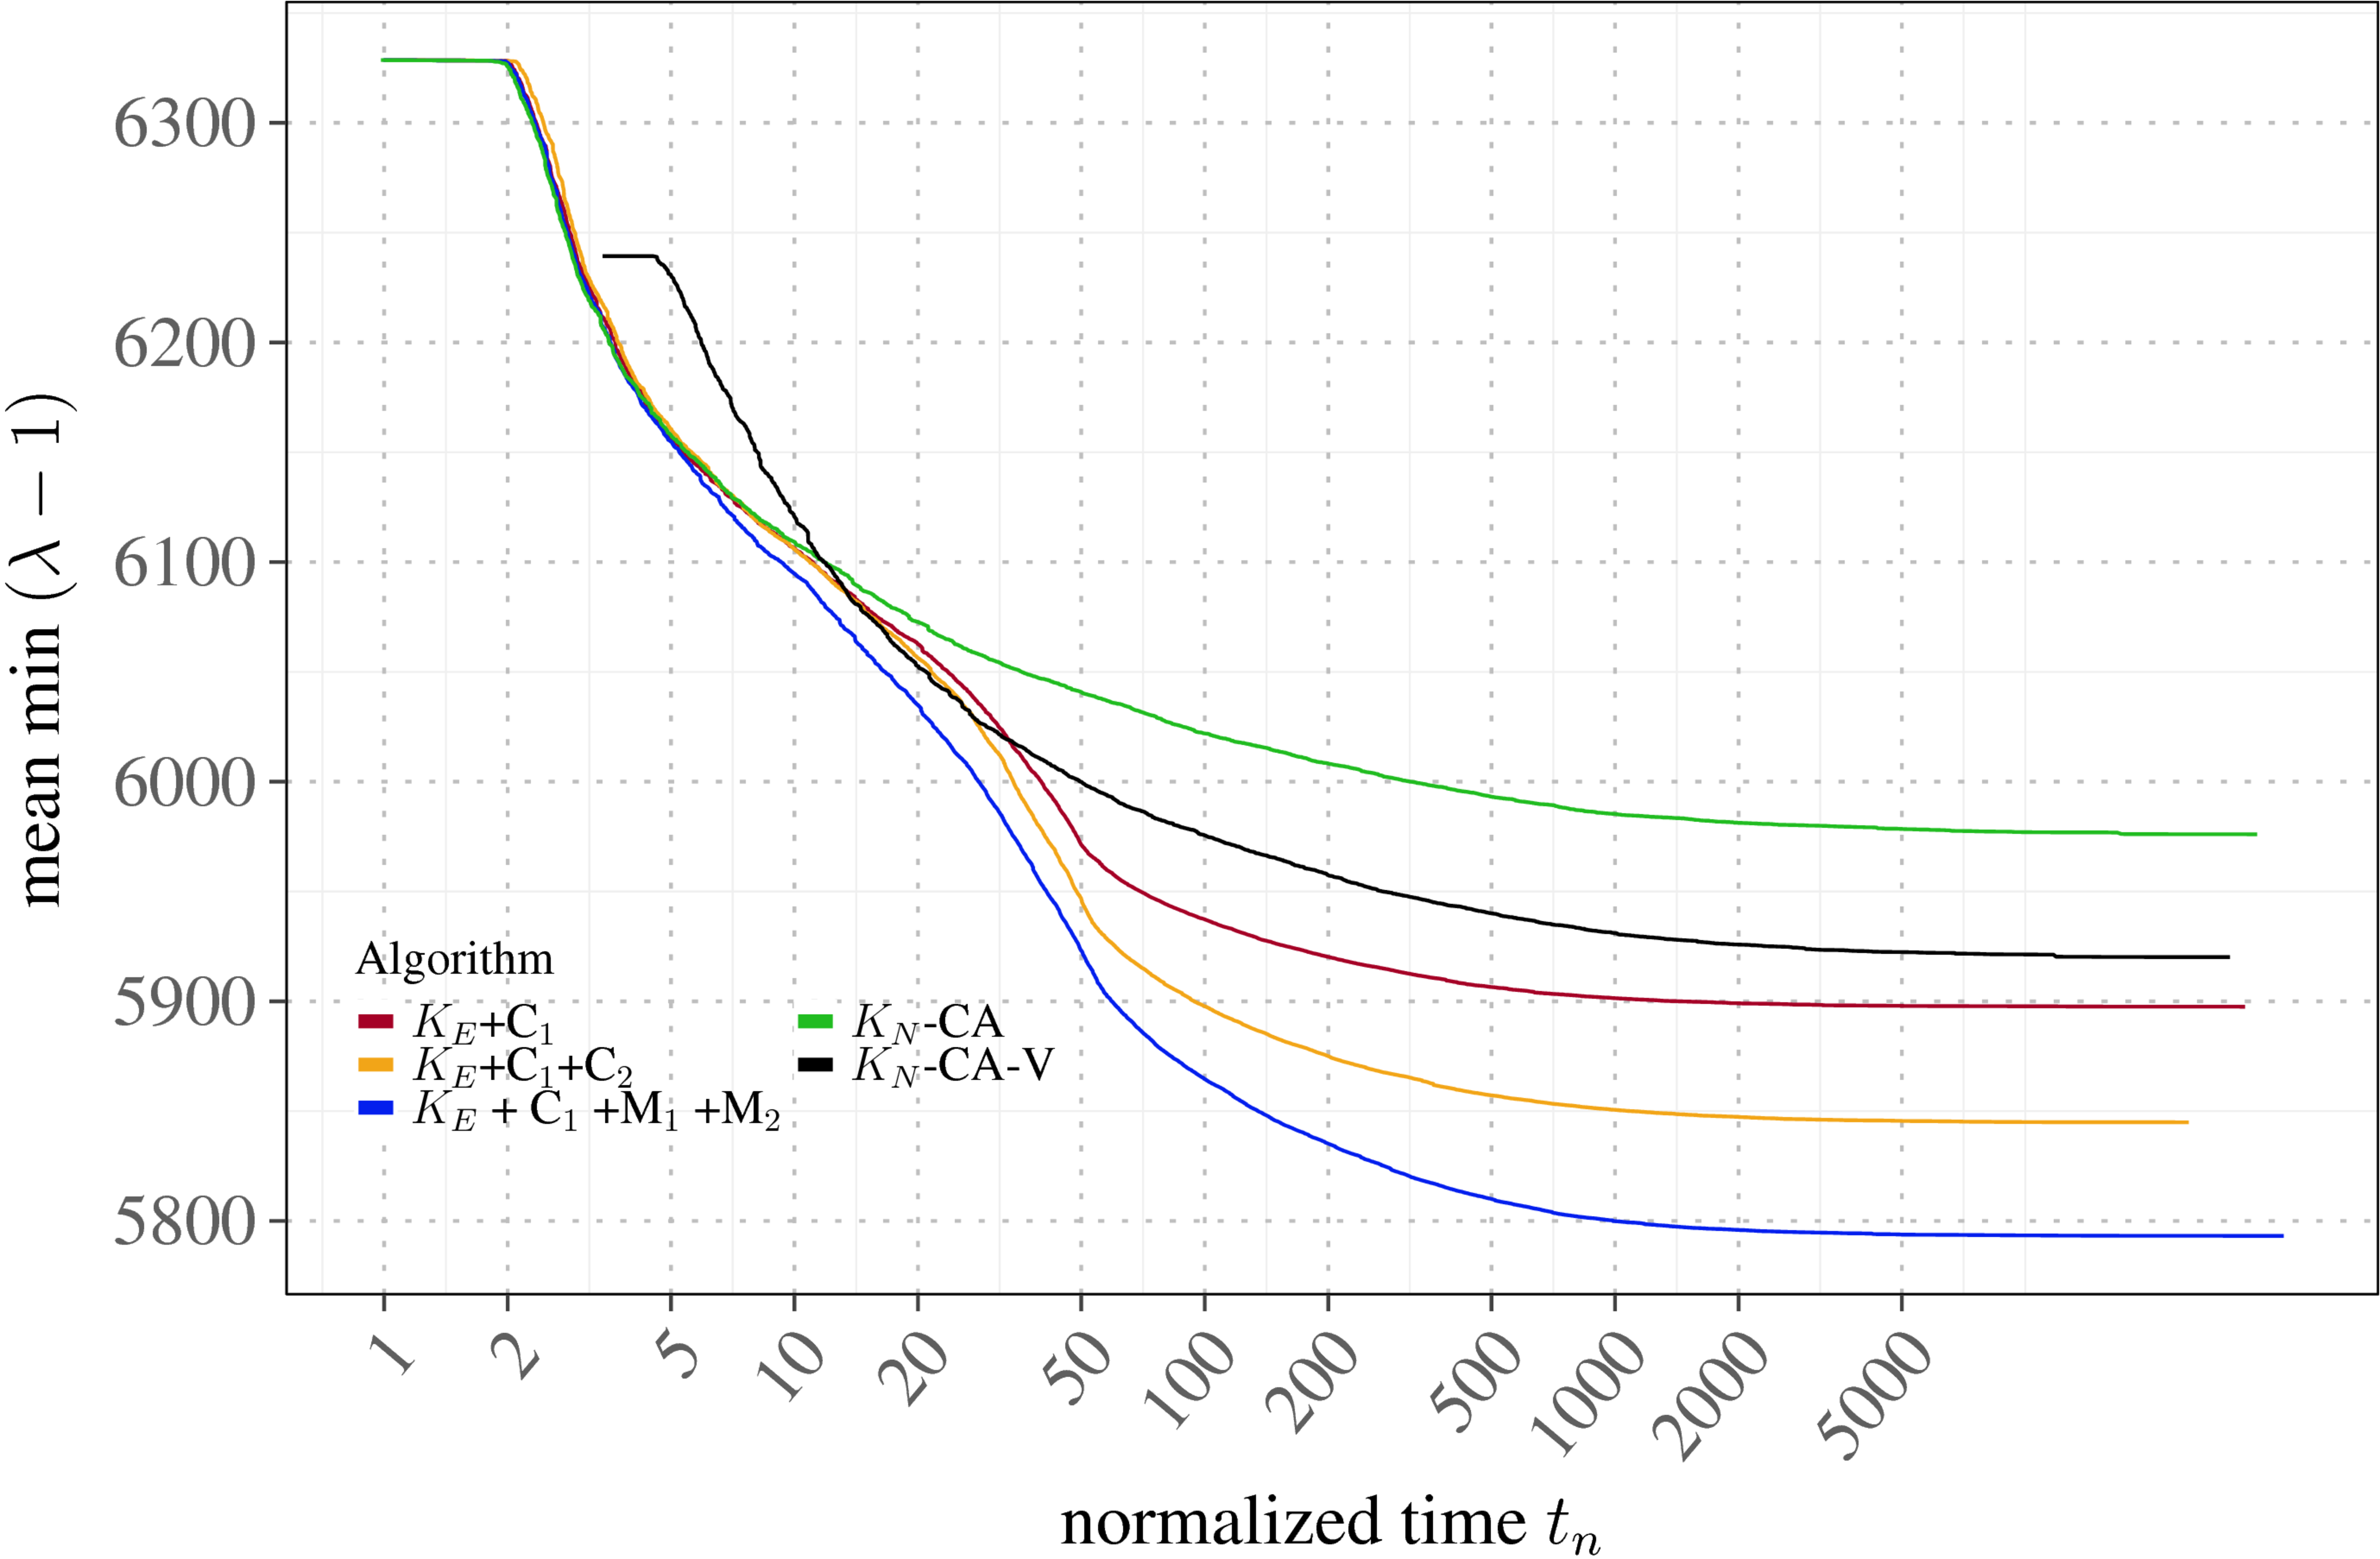
\includegraphics[width=\textwidth]{rnw/tuning_subset_plots/full_plot-1}
%<<full evaluation, fig=TRUE, echo=FALSE, height=4, width=6>>=
%source("/home/andre/server-home/temppap/R/plot_functions.R")
%source("/home/andre/server-home/temppap/R/final_preprocessing.R")

%data = 
%convergencePlot(automaticPlot(list("C1" = traditional_combine,
%                                   "C1C2" = random_combine,
%                                   "KaHyPar-CA" = kahypar_ca,
%                                   "KaHyPar-CA-V" = kahypar_ca_vcycle,
%                                   "C1M1M2" = trad_vcycle_mutate),
%                              baselineTime(traditional_combine)))
%@
\end{center}
In average all evolutionary operators are performing better. TODO TEXT
\end{figure}
% => Convergence split by k

\begin{figure}[H]
\caption{Benchmark subset split by k}
\begin{center}
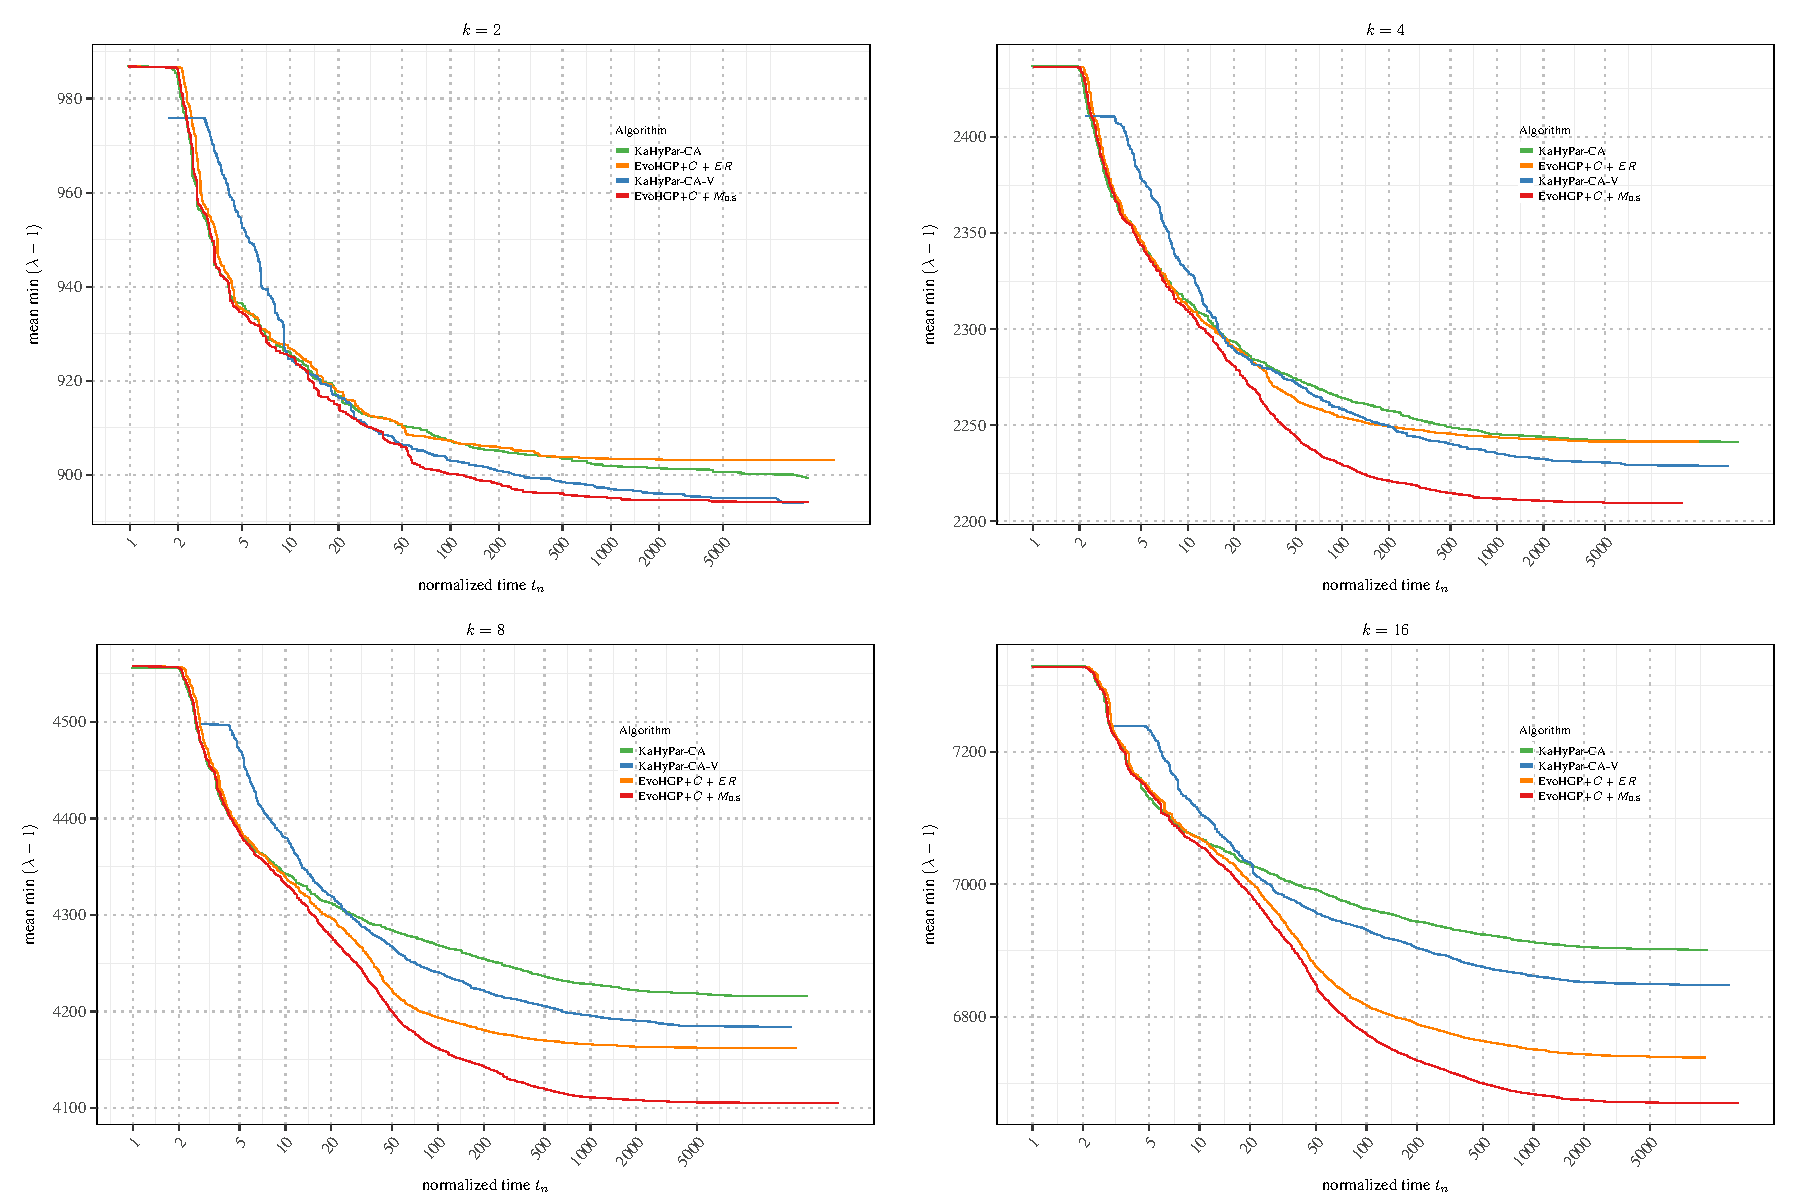
\includegraphics[width=\textwidth]{rnw/appendix_convergence-1}
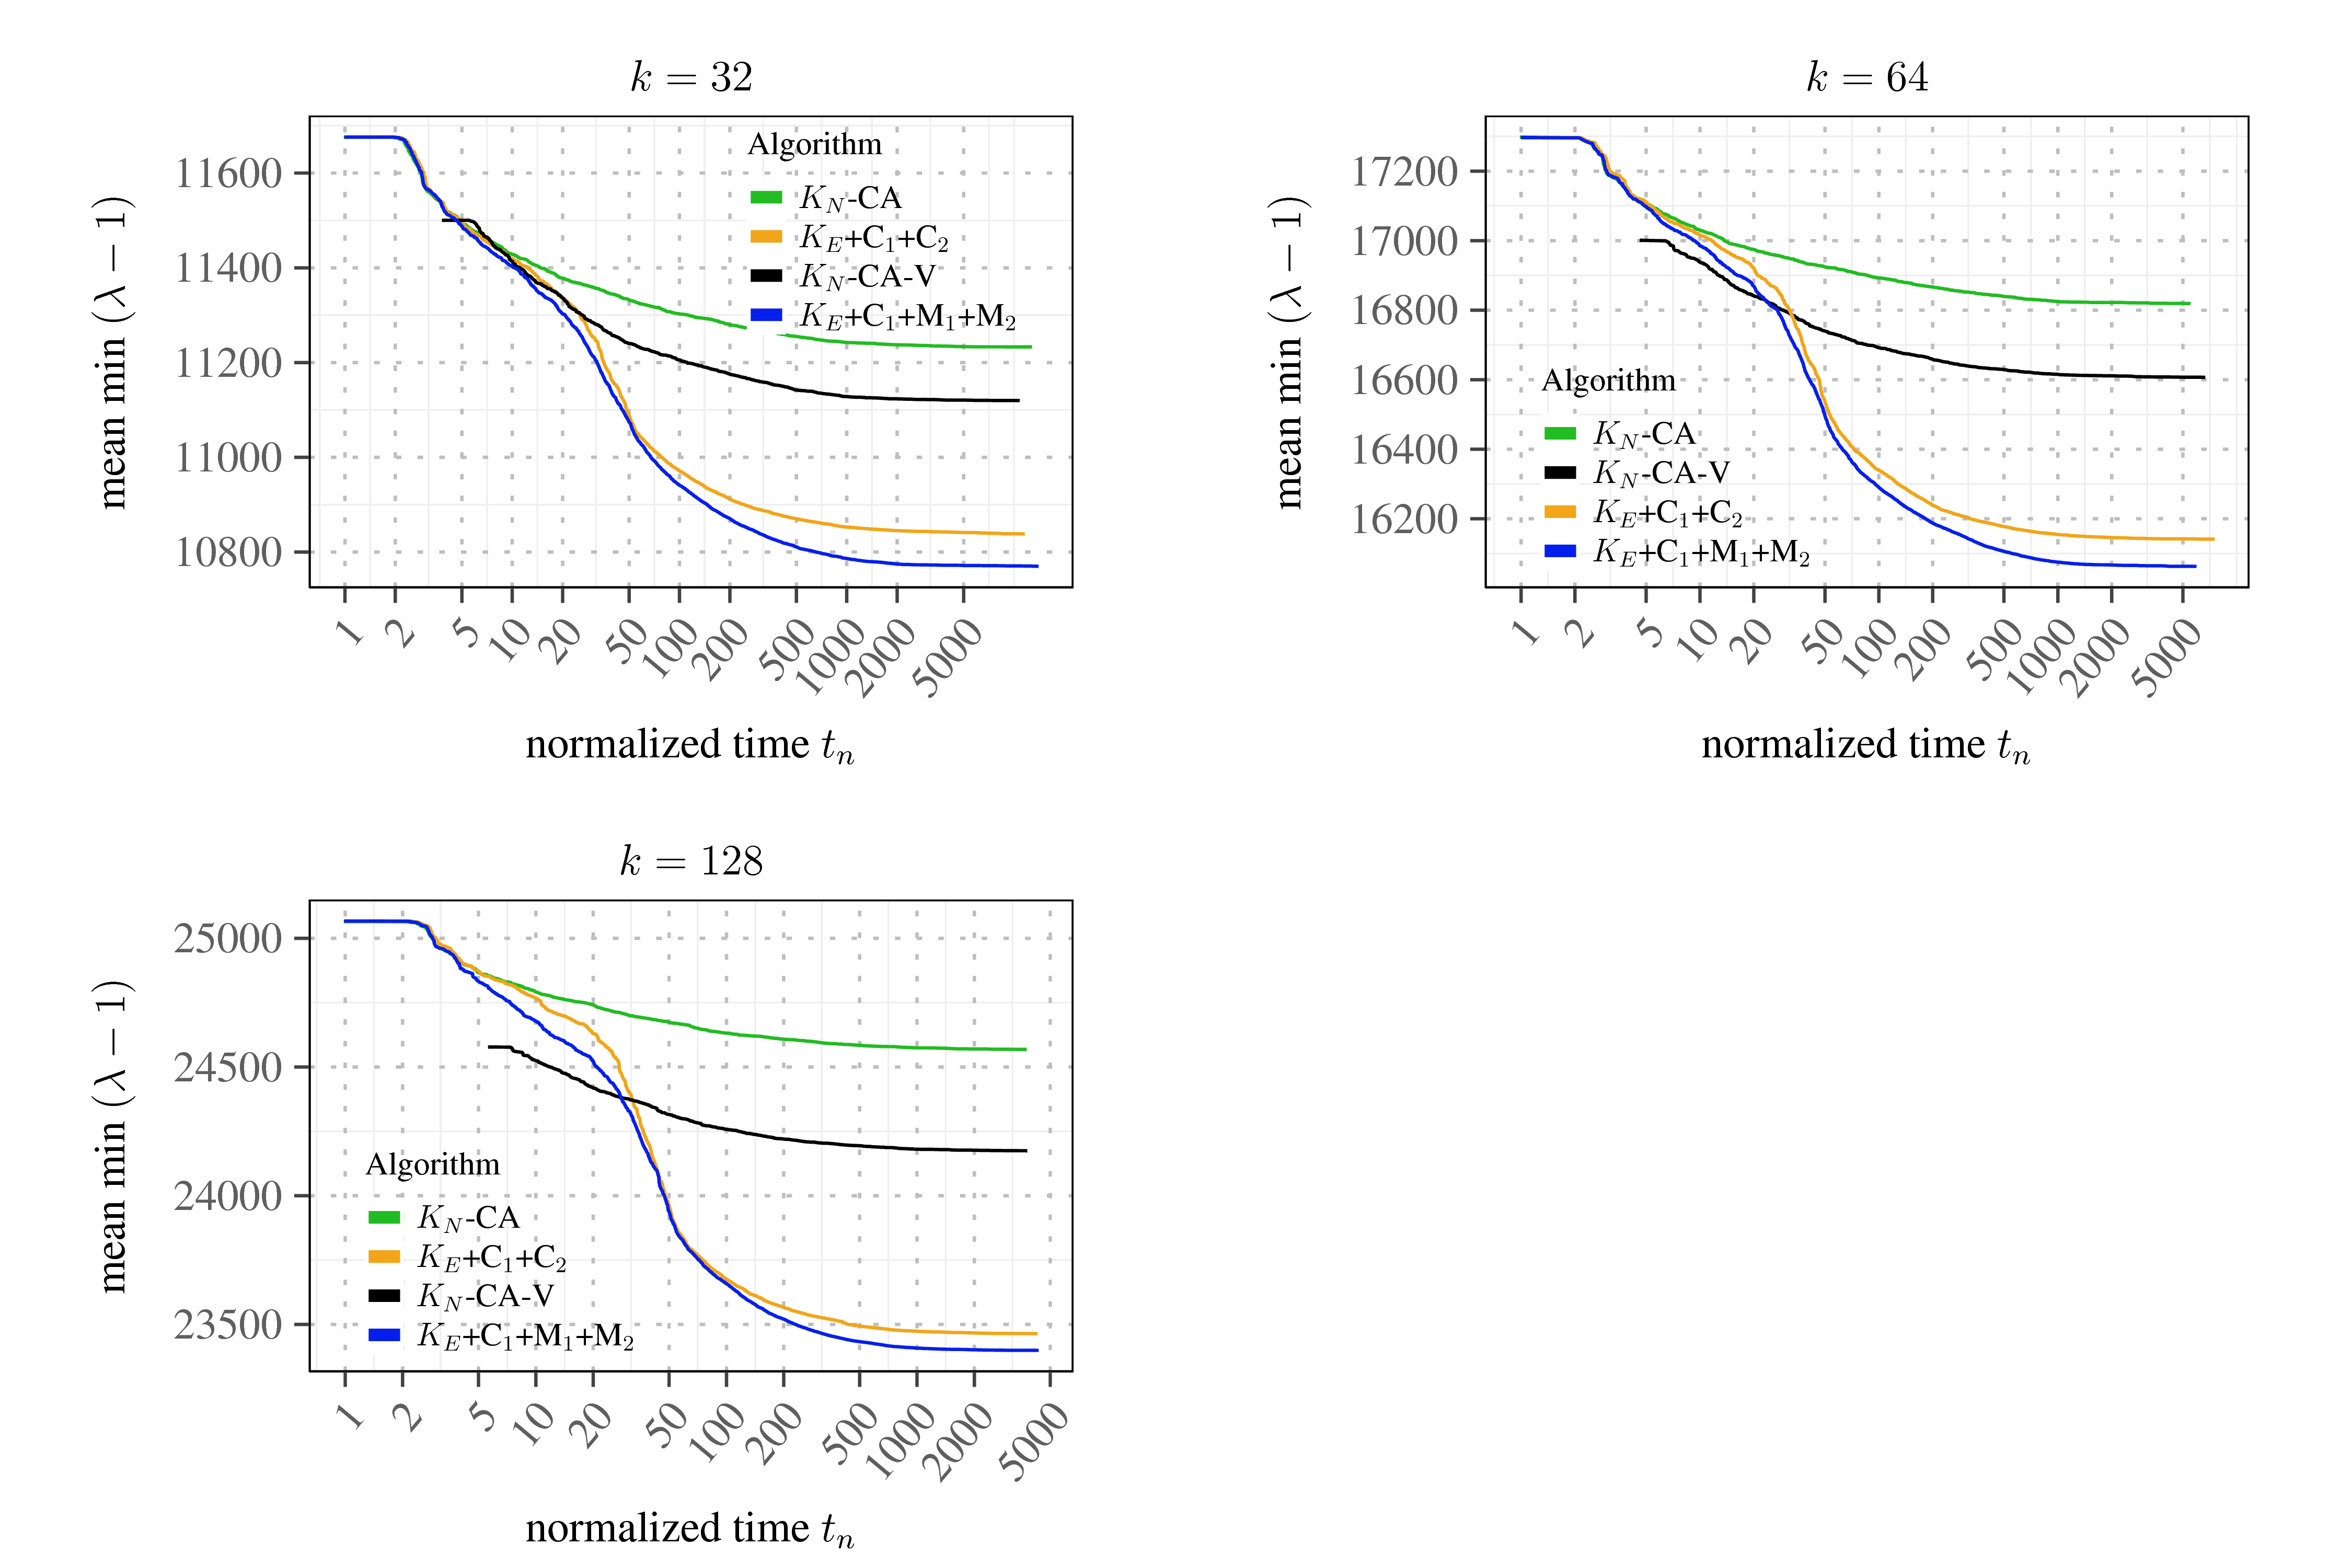
\includegraphics[width=\textwidth]{rnw/appendix_convergence-2}
%<<full evaluation, fig=TRUE, echo=FALSE, height=4, width=6>>=
%ks = c(2,4,8,16,32,64,128)
%for (k in ks) {
%  print(paste("k=",k))
%  data = automaticPlot(list("C1" = traditional_combine[traditional_combine$k == k,],
%                            "C1C2" = random_combine[random_combine$k == k,],
%                            "KaHyPar-CA" = kahypar_ca[kahypar_ca$k == k,],
%                            "KaHyPar-CA-V" = kahypar_ca_vcycle[kahypar_ca_vcycle$k == k,],
%                            "C1M1M2" = trad_vcycle_mutate[trad_vcycle_mutate$k == k,]),
%                       baselineTime(traditional_combine[traditional_combine$k == k,]))
%  print(convergencePlot(data,k))
%}
%@
\end{center}
The results for the specific k values should be described HERE
\end{figure}
% => Best results in how many instances
% => Table of improvements
\begin{figure}[t]


\centering
\vspace{0pt}
\captionof{table}{Connectivity improvement of the strongest configurations for KaHyPar-E}~\label{tbl:imp}
\begin{tabular}[H]{r||r|r||r|r}\label{tab:improvement}
% &  \multicolumn{4}{c}{Algorithms} \\ 
&\multicolumn{2}{c||}{KaHyPar-E+C1+C2} & \multicolumn{2}{c}{KaHyParE+C1+M1+M2} \\
$k$                     &                              KaHyPar-CA-V    & KaHyPar-CA &  KaHyPar-CA-V   & KaHyPar-CA  \\ 
                     \hline
                     \hline

all k &  1.7\% & 2.7\% & 2.2\% & 3.2\% \\
\hline
2&-0.2\% & 0.4\% & 0.2\% & 0.8\% \\
4& -0.2\% &0.3\% &0.9\% &1.3\%\\
8& 0.7\% &1.6\%& 1.9\% &2.7\%\\
16& 1.9\% &2.8\%& 2.6\%& 3.5\%\\
32& 2.9\% &3.9\%& 3.2\%& 4.2\%\\
64&  3.2\% &4.7\%& 3.4\% &4.8\%\\
128& 3.4\% &5.1\%& 3.3\% &5.0\% \\ 
\end{tabular}

%\vspace*{-.75cm}
\end{figure}
In table  \ref{tab:improvement} the average improvements of the two strongest configurations of KaHyPar-E are compared to KaHyPar-CA-V and KaHyPar-CA. 
The average improvements are then split by k. 

%ADD PERFORMANCE PLOT
\begin{figure}[H]
\begin{center}
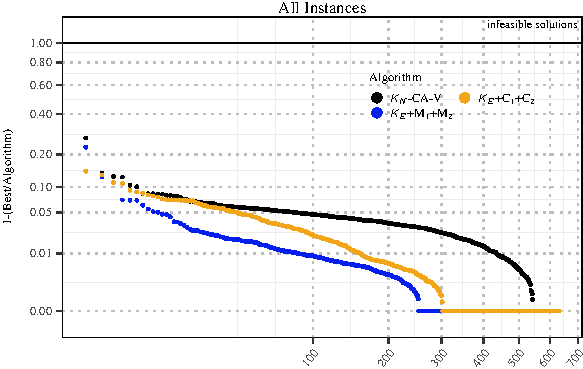
\includegraphics[width=\textwidth]{rnw/tuning_subset_plots/performance_plot_main-1}
\end{center}
\end{figure}





%%%%%%%%%%%%%%%%%%%%%%%%%%%%%%%%%%%%%%%%%%%%%%%%%%%%%%%%%%%%%%%%%%%%%%
\chapter{Discussion}
\section{Conclusion}
This thesis presents an evolutionary framework for KaHyPar resulting in a quality improvement for hypergraph partitions of up to 5\%. We used combine operators different from usual crossover approaches to detect and exploit good solution qualities in partitions, as well as mutation operations to increase the solution scope compared to KaHyPar. Additionally we created a diversity strategy applicable to hypergraphs for replacement. Our operators are heavily integrated into the standard procedure of KaHyPar, to the point where all operators make use of the multilevel partition steps provided by KaHyPar. This work is the first combination of multilevel and memetic algorithms in the field of hypergraph partitioning.
As expected of an evolutionary algorithm, the quality improvement needs multiple iterations to show significance. KaHyPar-E was designed with that mentality to improve the best possible solution for the partition of a hypergraph where the time constraint is of secondary relevance. 
\section{Future Work}
Currently KaHyPar-E is providing solution quality but no speedup for a single partition. Adding a layer of parallelization would allow a significant speedup by creating multiple individuals during an iteration. This should be realizable without greater effort due to the independence of the child and parent partitions. Another interesting approach is a time cost analysis for the different operators. There is a strong suggestion that the basic combine operator is significantly faster than a regular iteration in KaHyPar. If this suggestion is true, a faster population generation would be a valid approach to increase performance. Also the v-cycle mutation operator might turn out to be more beneficial if the number of cycles is increased. Other than that more sophistiacted selection strategies for parent selection as well as edge frequency might also be helpful. A more detailed analysis and exploitation of hypergraph structures may enhance the performance of the current evolutionary operators, or perhaps even inspire the addition of new operators.

\clearpage
\begin{appendix}
\chapter{Implementation Details}
\section{Software}
The source code was written in C++, using the C++11 version. The software was compiled by gcc-5.2+. The combine operators are implemented as a policy in the rater. These policies are meant to avoid overhead and control flow complexity during the coarsening, which is the most time consuming part of an iteration in KaHyPar. An action element is attached to each iteration, containing the necessary requirements for each of the different operation. These requirements activate or deactivate 
initial partitioning or the use of parent information during the coarsening, depending on the action performed. Edge frequency and stable net removal use the same baseline vector containing the amount of cut edges from X partitions. 
% Data Structures etc..

\end{appendix}
%%%%%%%%%%%%%%%%%%%%%%%%%%%%%%%%%%%%%%%%%%%%%%%%%%%%%%%%%%%%%%%%%%%%%%
\bibliographystyle{gerplain}
\bibliography{literatur}
\end{document}
